% Options for packages loaded elsewhere
\PassOptionsToPackage{unicode}{hyperref}
\PassOptionsToPackage{hyphens}{url}
\PassOptionsToPackage{dvipsnames,svgnames,x11names}{xcolor}
%
\documentclass[
  letterpaper,
  DIV=11,
  numbers=noendperiod]{scrreprt}

\usepackage{amsmath,amssymb}
\usepackage{iftex}
\ifPDFTeX
  \usepackage[T1]{fontenc}
  \usepackage[utf8]{inputenc}
  \usepackage{textcomp} % provide euro and other symbols
\else % if luatex or xetex
  \usepackage{unicode-math}
  \defaultfontfeatures{Scale=MatchLowercase}
  \defaultfontfeatures[\rmfamily]{Ligatures=TeX,Scale=1}
\fi
\usepackage{lmodern}
\ifPDFTeX\else  
    % xetex/luatex font selection
\fi
% Use upquote if available, for straight quotes in verbatim environments
\IfFileExists{upquote.sty}{\usepackage{upquote}}{}
\IfFileExists{microtype.sty}{% use microtype if available
  \usepackage[]{microtype}
  \UseMicrotypeSet[protrusion]{basicmath} % disable protrusion for tt fonts
}{}
\makeatletter
\@ifundefined{KOMAClassName}{% if non-KOMA class
  \IfFileExists{parskip.sty}{%
    \usepackage{parskip}
  }{% else
    \setlength{\parindent}{0pt}
    \setlength{\parskip}{6pt plus 2pt minus 1pt}}
}{% if KOMA class
  \KOMAoptions{parskip=half}}
\makeatother
\usepackage{xcolor}
\setlength{\emergencystretch}{3em} % prevent overfull lines
\setcounter{secnumdepth}{5}
% Make \paragraph and \subparagraph free-standing
\ifx\paragraph\undefined\else
  \let\oldparagraph\paragraph
  \renewcommand{\paragraph}[1]{\oldparagraph{#1}\mbox{}}
\fi
\ifx\subparagraph\undefined\else
  \let\oldsubparagraph\subparagraph
  \renewcommand{\subparagraph}[1]{\oldsubparagraph{#1}\mbox{}}
\fi

\usepackage{color}
\usepackage{fancyvrb}
\newcommand{\VerbBar}{|}
\newcommand{\VERB}{\Verb[commandchars=\\\{\}]}
\DefineVerbatimEnvironment{Highlighting}{Verbatim}{commandchars=\\\{\}}
% Add ',fontsize=\small' for more characters per line
\usepackage{framed}
\definecolor{shadecolor}{RGB}{241,243,245}
\newenvironment{Shaded}{\begin{snugshade}}{\end{snugshade}}
\newcommand{\AlertTok}[1]{\textcolor[rgb]{0.68,0.00,0.00}{#1}}
\newcommand{\AnnotationTok}[1]{\textcolor[rgb]{0.37,0.37,0.37}{#1}}
\newcommand{\AttributeTok}[1]{\textcolor[rgb]{0.40,0.45,0.13}{#1}}
\newcommand{\BaseNTok}[1]{\textcolor[rgb]{0.68,0.00,0.00}{#1}}
\newcommand{\BuiltInTok}[1]{\textcolor[rgb]{0.00,0.23,0.31}{#1}}
\newcommand{\CharTok}[1]{\textcolor[rgb]{0.13,0.47,0.30}{#1}}
\newcommand{\CommentTok}[1]{\textcolor[rgb]{0.37,0.37,0.37}{#1}}
\newcommand{\CommentVarTok}[1]{\textcolor[rgb]{0.37,0.37,0.37}{\textit{#1}}}
\newcommand{\ConstantTok}[1]{\textcolor[rgb]{0.56,0.35,0.01}{#1}}
\newcommand{\ControlFlowTok}[1]{\textcolor[rgb]{0.00,0.23,0.31}{#1}}
\newcommand{\DataTypeTok}[1]{\textcolor[rgb]{0.68,0.00,0.00}{#1}}
\newcommand{\DecValTok}[1]{\textcolor[rgb]{0.68,0.00,0.00}{#1}}
\newcommand{\DocumentationTok}[1]{\textcolor[rgb]{0.37,0.37,0.37}{\textit{#1}}}
\newcommand{\ErrorTok}[1]{\textcolor[rgb]{0.68,0.00,0.00}{#1}}
\newcommand{\ExtensionTok}[1]{\textcolor[rgb]{0.00,0.23,0.31}{#1}}
\newcommand{\FloatTok}[1]{\textcolor[rgb]{0.68,0.00,0.00}{#1}}
\newcommand{\FunctionTok}[1]{\textcolor[rgb]{0.28,0.35,0.67}{#1}}
\newcommand{\ImportTok}[1]{\textcolor[rgb]{0.00,0.46,0.62}{#1}}
\newcommand{\InformationTok}[1]{\textcolor[rgb]{0.37,0.37,0.37}{#1}}
\newcommand{\KeywordTok}[1]{\textcolor[rgb]{0.00,0.23,0.31}{#1}}
\newcommand{\NormalTok}[1]{\textcolor[rgb]{0.00,0.23,0.31}{#1}}
\newcommand{\OperatorTok}[1]{\textcolor[rgb]{0.37,0.37,0.37}{#1}}
\newcommand{\OtherTok}[1]{\textcolor[rgb]{0.00,0.23,0.31}{#1}}
\newcommand{\PreprocessorTok}[1]{\textcolor[rgb]{0.68,0.00,0.00}{#1}}
\newcommand{\RegionMarkerTok}[1]{\textcolor[rgb]{0.00,0.23,0.31}{#1}}
\newcommand{\SpecialCharTok}[1]{\textcolor[rgb]{0.37,0.37,0.37}{#1}}
\newcommand{\SpecialStringTok}[1]{\textcolor[rgb]{0.13,0.47,0.30}{#1}}
\newcommand{\StringTok}[1]{\textcolor[rgb]{0.13,0.47,0.30}{#1}}
\newcommand{\VariableTok}[1]{\textcolor[rgb]{0.07,0.07,0.07}{#1}}
\newcommand{\VerbatimStringTok}[1]{\textcolor[rgb]{0.13,0.47,0.30}{#1}}
\newcommand{\WarningTok}[1]{\textcolor[rgb]{0.37,0.37,0.37}{\textit{#1}}}

\providecommand{\tightlist}{%
  \setlength{\itemsep}{0pt}\setlength{\parskip}{0pt}}\usepackage{longtable,booktabs,array}
\usepackage{calc} % for calculating minipage widths
% Correct order of tables after \paragraph or \subparagraph
\usepackage{etoolbox}
\makeatletter
\patchcmd\longtable{\par}{\if@noskipsec\mbox{}\fi\par}{}{}
\makeatother
% Allow footnotes in longtable head/foot
\IfFileExists{footnotehyper.sty}{\usepackage{footnotehyper}}{\usepackage{footnote}}
\makesavenoteenv{longtable}
\usepackage{graphicx}
\makeatletter
\def\maxwidth{\ifdim\Gin@nat@width>\linewidth\linewidth\else\Gin@nat@width\fi}
\def\maxheight{\ifdim\Gin@nat@height>\textheight\textheight\else\Gin@nat@height\fi}
\makeatother
% Scale images if necessary, so that they will not overflow the page
% margins by default, and it is still possible to overwrite the defaults
% using explicit options in \includegraphics[width, height, ...]{}
\setkeys{Gin}{width=\maxwidth,height=\maxheight,keepaspectratio}
% Set default figure placement to htbp
\makeatletter
\def\fps@figure{htbp}
\makeatother
\newlength{\cslhangindent}
\setlength{\cslhangindent}{1.5em}
\newlength{\csllabelwidth}
\setlength{\csllabelwidth}{3em}
\newlength{\cslentryspacingunit} % times entry-spacing
\setlength{\cslentryspacingunit}{\parskip}
\newenvironment{CSLReferences}[2] % #1 hanging-ident, #2 entry spacing
 {% don't indent paragraphs
  \setlength{\parindent}{0pt}
  % turn on hanging indent if param 1 is 1
  \ifodd #1
  \let\oldpar\par
  \def\par{\hangindent=\cslhangindent\oldpar}
  \fi
  % set entry spacing
  \setlength{\parskip}{#2\cslentryspacingunit}
 }%
 {}
\usepackage{calc}
\newcommand{\CSLBlock}[1]{#1\hfill\break}
\newcommand{\CSLLeftMargin}[1]{\parbox[t]{\csllabelwidth}{#1}}
\newcommand{\CSLRightInline}[1]{\parbox[t]{\linewidth - \csllabelwidth}{#1}\break}
\newcommand{\CSLIndent}[1]{\hspace{\cslhangindent}#1}

\KOMAoption{captions}{tableheading}
\makeatletter
\makeatother
\makeatletter
\@ifpackageloaded{bookmark}{}{\usepackage{bookmark}}
\makeatother
\makeatletter
\@ifpackageloaded{caption}{}{\usepackage{caption}}
\AtBeginDocument{%
\ifdefined\contentsname
  \renewcommand*\contentsname{Table of contents}
\else
  \newcommand\contentsname{Table of contents}
\fi
\ifdefined\listfigurename
  \renewcommand*\listfigurename{List of Figures}
\else
  \newcommand\listfigurename{List of Figures}
\fi
\ifdefined\listtablename
  \renewcommand*\listtablename{List of Tables}
\else
  \newcommand\listtablename{List of Tables}
\fi
\ifdefined\figurename
  \renewcommand*\figurename{Figure}
\else
  \newcommand\figurename{Figure}
\fi
\ifdefined\tablename
  \renewcommand*\tablename{Table}
\else
  \newcommand\tablename{Table}
\fi
}
\@ifpackageloaded{float}{}{\usepackage{float}}
\floatstyle{ruled}
\@ifundefined{c@chapter}{\newfloat{codelisting}{h}{lop}}{\newfloat{codelisting}{h}{lop}[chapter]}
\floatname{codelisting}{Listing}
\newcommand*\listoflistings{\listof{codelisting}{List of Listings}}
\usepackage{amsthm}
\theoremstyle{definition}
\newtheorem{example}{Example}[chapter]
\theoremstyle{definition}
\newtheorem{definition}{Definition}[chapter]
\theoremstyle{remark}
\AtBeginDocument{\renewcommand*{\proofname}{Proof}}
\newtheorem*{remark}{Remark}
\newtheorem*{solution}{Solution}
\makeatother
\makeatletter
\@ifpackageloaded{caption}{}{\usepackage{caption}}
\@ifpackageloaded{subcaption}{}{\usepackage{subcaption}}
\makeatother
\makeatletter
\@ifpackageloaded{tcolorbox}{}{\usepackage[skins,breakable]{tcolorbox}}
\makeatother
\makeatletter
\@ifundefined{shadecolor}{\definecolor{shadecolor}{rgb}{.97, .97, .97}}
\makeatother
\makeatletter
\makeatother
\makeatletter
\makeatother
\ifLuaTeX
  \usepackage{selnolig}  % disable illegal ligatures
\fi
\IfFileExists{bookmark.sty}{\usepackage{bookmark}}{\usepackage{hyperref}}
\IfFileExists{xurl.sty}{\usepackage{xurl}}{} % add URL line breaks if available
\urlstyle{same} % disable monospaced font for URLs
\hypersetup{
  pdftitle={Introdução à Inferência Bayesiana},
  pdfauthor={James D Santos},
  colorlinks=true,
  linkcolor={blue},
  filecolor={Maroon},
  citecolor={Blue},
  urlcolor={Blue},
  pdfcreator={LaTeX via pandoc}}

\title{Introdução à Inferência Bayesiana}
\author{James D Santos}
\date{2023-10-03}

\begin{document}
\maketitle
\ifdefined\Shaded\renewenvironment{Shaded}{\begin{tcolorbox}[frame hidden, enhanced, sharp corners, borderline west={3pt}{0pt}{shadecolor}, boxrule=0pt, breakable, interior hidden]}{\end{tcolorbox}}\fi

\renewcommand*\contentsname{Table of contents}
{
\hypersetup{linkcolor=}
\setcounter{tocdepth}{2}
\tableofcontents
}
\bookmarksetup{startatroot}

\hypertarget{preface}{%
\chapter*{Preface}\label{preface}}
\addcontentsline{toc}{chapter}{Preface}

\markboth{Preface}{Preface}

Este material foi criado para a disciplina Introdução à Inferência
Bayesiana, do curso de bacharelado em Estatística, da Universidade
Federal do Amazonas.

\bookmarksetup{startatroot}

\hypertarget{section}{%
\chapter{}\label{section}}

\bookmarksetup{startatroot}

\hypertarget{aula-1---introduuxe7uxe3o}{%
\chapter{Aula 1 - Introdução}\label{aula-1---introduuxe7uxe3o}}

Os objetivos desta aula são:

\begin{enumerate}
\def\labelenumi{\arabic{enumi}.}
\tightlist
\item
  Apresentar a notação
\item
  Explicar sobre as fontes de informação
\item
  Apresentar as inferências básicas
\item
  Discutir como se dá o processo de elicitação de prioris
\end{enumerate}

\hypertarget{notauxe7uxe3o}{%
\section{Notação}\label{notauxe7uxe3o}}

Variáveis aleatórias cujo valor podem ser observados serão denotadas por
letras maiúsculas. Exemplos:

\begin{itemize}
\item
  \(X\) é número de acidentes diários na Avenida Torquato Tapajós
\item
  \(Y\) é o nível máximo diário do Rio Negro
\end{itemize}

Valores observados de variáveis aleatórias serão denotados pela
respectiva letra minúscula.

Parâmetros serão considerados aleatórios, mas serão representados por
letras gregas minúsculas, como \(\theta\), \(\lambda\), etc.

Vetores aleatórios serão representados por letras em negrito. Exemplos:

\begin{itemize}
\item
  \(\mathbf{X} = \{X_1 , \ldots , X_n \}\) é um vetor de variáveis
  aleatórias.
\item
  \(\mathbf{x} = \{x_1 ,\ldots , x_n \}\) é um vetor observado de
  variáveis aleatórias.
\item
  \(\theta=\{\alpha,\beta\}\) é um vetor de parâmetros.
\end{itemize}

\begin{definition}[]\protect\hypertarget{def-Suporte}{}\label{def-Suporte}

O suporte de uma variável aleatória é o conjunto de todos os seus
possíveis valores. Quando necessário, o suporte de variáveis aleatórias
são representada pela versão caligráfica de sua letra correspondente.

Exemplos: o suporte de \(X\) é \(\mathcal{X}\) ; o suporte de Y é
\(\mathcal{Y}\) ; o suporte de \(Z\) é \(\mathcal{Z}\).

\end{definition}

\begin{definition}[]\protect\hypertarget{def-Espaco}{}\label{def-Espaco}

O espaço paramétrico é o conjunto de todos os possíveis valores do
parâmetro. Eles são representados pela versão maiúscula da letra grega
utilizada para seu respectivo parâmetro.

Exemplo: o espaço paramétrico do parâmetro \(\theta\) é representado por
\(\Theta\).

\end{definition}

Tanto a função de densidade quanto a de probabilidade serão denotadas
por funções começando com letras minúsculas. Por exemplo,

\[f(x|\lambda)=\lambda e^{-\lambda x}\] onde \(x,\lambda>0\) é a
densidade da distribuição exponencial, enquanto que

\[p(x|\lambda)=\frac{e^{-\lambda}\lambda^x}{x!}\] com \(x\in\mathbb{N}\)
e \(\lambda >0\) é a é a função de probabilidade da distribuição
Poisson.

\hypertarget{fontes-de-informauxe7uxe3o}{%
\section{Fontes de informação}\label{fontes-de-informauxe7uxe3o}}

\hypertarget{a-funuxe7uxe3o-de-verossimilhanuxe7a}{%
\subsection{A função de
verossimilhança}\label{a-funuxe7uxe3o-de-verossimilhanuxe7a}}

Seja \(\mathbf{x} = \{x_1 , \ldots , x_n \}\) uma amostra observada.
Supomos que \(\mathbf{x}\) é uma das possíveis amostras das variáveis
aleatórias \(\mathbf{X} = \{X_1 , \ldots , X_n \}\). Supomos ainda que
\(X\sim F (.|\theta)\). Assim, condicionada ao conhecimento de
\(\theta\), a distribuição da amostra está completamente especificada.

::: \{\#def-Funcao de verossimilhanca\} Para \(\mathbf{x}\) fixado, a
função \[L:\Theta\Rightarrow [0,\infty)\] é denominada verossimilhança.
:::

Sua interpretação é a seguinte: para \(\theta_1,\theta_2\in\Theta\), se

\[L(\theta_1)>L(\theta_2),\] dizemos que \(\theta_1\) é mais verossímil
que \(\theta_2\). Isto porque a probabilidade de observar uma amostra na
vizinhança de \(\mathbf{x}\) é maior se considerarmos que \(\theta_1\) é
o valor do parâmetro. A verossimilhança é uma das fontes de informação
utilizada na inferência bayesiana (e a única fonte da inferência
frequentista).

\begin{example}[]\protect\hypertarget{exm-}{}\label{exm-}

Considere uma amostra de 30 variáveis aleatórias independentes com
distribuição Poisson(\(\theta\)). Neste caso, a função de
verossimilhança será
\[L(\theta)=\frac{e^{-30\theta}\theta^{\sum_{i=1}^{30}x_i}}{\prod_{i=1}^{30}x_i!}.\]
Vamos simular uma amostra de tamanho 30 deste modelo (o valor de
\(\theta\) será omisso de propósito)

\begin{Shaded}
\begin{Highlighting}[]
\NormalTok{x }\OtherTok{\textless{}{-}} \FunctionTok{rpois}\NormalTok{(}\DecValTok{30}\NormalTok{,theta)}
\NormalTok{x}
\end{Highlighting}
\end{Shaded}

\begin{verbatim}
 [1] 2 4 2 5 6 0 3 5 3 3 6 3 4 3 1 5 2 0 2 6 5 4 3 8 4 4 3 3 2 1
\end{verbatim}

A próxima figura mostra os valores da função de verossimilhança para
vários valores de \(\theta\) para a amostra observada.

\begin{Shaded}
\begin{Highlighting}[]
\CommentTok{\# função de verossimilhança}
\NormalTok{vero }\OtherTok{\textless{}{-}} \ControlFlowTok{function}\NormalTok{(q)\{}
  \FunctionTok{sapply}\NormalTok{ ( q, }\ControlFlowTok{function}\NormalTok{(q) }\FunctionTok{prod}\NormalTok{(}\FunctionTok{dpois}\NormalTok{(x, q)) ) }
\NormalTok{\} }

\CommentTok{\# gráfico da função de verossimilhança}
\NormalTok{oo }\OtherTok{\textless{}{-}} \FunctionTok{par}\NormalTok{( }\AttributeTok{cex =} \FloatTok{1.2}\NormalTok{)}
\FunctionTok{curve}\NormalTok{( }\FunctionTok{vero}\NormalTok{(x),}\DecValTok{2}\NormalTok{,}\FloatTok{4.5}\NormalTok{, }\AttributeTok{xlab =} \FunctionTok{expression}\NormalTok{(theta), }\AttributeTok{ylab =} \FunctionTok{expression}\NormalTok{( }\FunctionTok{L}\NormalTok{(theta)) , }\AttributeTok{lwd =} \DecValTok{2}\NormalTok{)}
\end{Highlighting}
\end{Shaded}

\begin{figure}[H]

{\centering 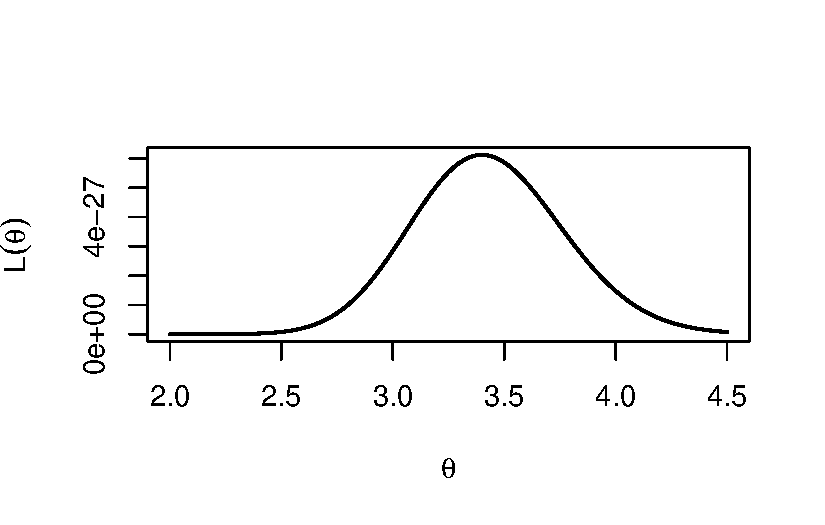
\includegraphics{intro_files/figure-pdf/unnamed-chunk-3-1.pdf}

}

\end{figure}

\begin{Shaded}
\begin{Highlighting}[]
\FunctionTok{par}\NormalTok{(oo)}
\end{Highlighting}
\end{Shaded}

Podemos notar que o valores mais verossímeis para \(\theta\) estão entre
2 e 4. Podemos ainda procurar o valor mais verossímil, denominado
\textbf{estimativa de máxima verossimilhança (emv).} Pode-se mostrar,
utilizando cálculo diferencial, que este valor é equivalente à média
amostral. Contudo, com o objetivo de utilizar ao máximo o poder
computacional que temos disponível, vamos encontrar esse valor
utilizando a função \texttt{optimize}.

\begin{Shaded}
\begin{Highlighting}[]
\CommentTok{\# menos o logaritmo da função de verossimilhança}
\NormalTok{lvero }\OtherTok{\textless{}{-}} \ControlFlowTok{function}\NormalTok{(q) }\SpecialCharTok{{-}}\FunctionTok{log}\NormalTok{( }\FunctionTok{vero}\NormalTok{(q))}

\CommentTok{\# encontrando a emv:}
\FunctionTok{optimise}\NormalTok{(lvero, }\FunctionTok{c}\NormalTok{(}\DecValTok{2}\NormalTok{,}\DecValTok{4}\NormalTok{))}
\end{Highlighting}
\end{Shaded}

\begin{verbatim}
$minimum
[1] 3.399981

$objective
[1] 60.35731
\end{verbatim}

O valor 2,6 é a estimativa de verossimilhança (este é o valor exato da
média amotral). Sob o ponto de vista frequentista, esta seria a nossa
estiamtiva para o valor de \(\theta\).

\end{example}

\hypertarget{a-distribuiuxe7uxe3o-a-priori}{%
\subsection{A distribuição a
priori}\label{a-distribuiuxe7uxe3o-a-priori}}

Sob o ponto de vista bayesiano, a informação existente sobre \(\theta\)
antes da observação da amostra deve ser levada em consideração. Isto é
feito traduzindo tal informação em termos de probabilidades.

\begin{definition}[]\protect\hypertarget{def-}{}\label{def-}

A distribuição de \(\theta\) é denominada \textbf{distribuição a
priori}.

\end{definition}

Os parâmetros da distribuição \textbf{a priori} são denominados hiper
parâmetros.

As distribuições a priori : * agregam o conhecimento sobre parâmetro
antes da observação da amostra (tal conhecimento pode ter sido gerado de
uma amostra prévia). * podem ser muito ou pouco informativas, dependendo
do grau de crença sobre os valores em particular do espaço paramétrico.
Em geral isto é feito alterando a variância da distribuição:

\[\hbox{variância}=\frac{1}{\hbox{precisão}}\]

\hypertarget{reunindo-as-fontes-de-informauxe7uxe3o---distribuiuxe7uxe3o-a-posteriori}{%
\subsection{Reunindo as fontes de informação - distribuição a
posteriori}\label{reunindo-as-fontes-de-informauxe7uxe3o---distribuiuxe7uxe3o-a-posteriori}}

Sejam \(f(\boldsymbol{\theta})\) a densidade/função \textit{a priori}
para \(\boldsymbol{\theta}\) e \(L(\boldsymbol{\theta})\) a função de
verossimilhança.

Como \(\boldsymbol{\theta}\) é considerado aleatório, podemos analisar
sua distribuição \textbf{após} observar a amostra \(\boldsymbol{x}\), ou
seja \[\boldsymbol{\theta}|\boldsymbol{x}.\]

Esta distribuição é denominada \textit{posteriori}

::: \{\#thm-Teorema de Bayes\}

Seja \(\boldsymbol{x}\) uma amostra observada. Considere a priori
\(\theta\sim f(\theta)\) e a verossimilhança \(L(\theta)\). Então a
função de densidade (ou probabilidade) \textit{a posteriori} de
\(\theta|\boldsymbol{x}\) é dada por
\[f(\theta|\boldsymbol{x})=\frac{L(\theta)f(\theta)}{f(\boldsymbol{x})}.\]
O denominador é denominado distribuição preditiva, sendo igual a
\[f(\boldsymbol{x})=\sum_{\theta\in \Theta}L(\theta)f(\theta),\] se
\(\theta\) é v.a. discreta ou
\[f(\boldsymbol{x})=\int_{\Theta}L(\theta)f(\theta)d\theta\] se
\(\theta\) é v.a. contínua. :::

\hypertarget{inferuxeancia-estatuxedstica}{%
\section{Inferência estatística}\label{inferuxeancia-estatuxedstica}}

Denominamos por estatística qualquer função da amostra. Utilizamos
estatísticas para fazer as seguintes inferências:

\begin{itemize}
\item
  \emph{Estimação pontual}: trata-se de uma estatística com o objetivo
  de inferir o valor de \(\theta\). Tal estatística é denominada
  \textbf{estimador}.
\item
  \emph{Estimação por região}: trata-se de uma estatística, digamos
  \(T(\boldsymbol{X})\), com o objetivo de cobrir o valor de \(\theta\),
  ou seja, fazer a inferência \(\theta\in T(\boldsymbol{X})\). As
  estimações intervalares são as mais comuns, nas quais
  \(T(\boldsymbol{X})=(L(\boldsymbol{X}),U(\boldsymbol{X}))\).
\item
  \emph{Testes de hipóteses}: são estatísticas construídas para decidir
  se aceitamos a afirmação (hipótese) \(H:\theta\in \Theta_0\), onde
  \(\Theta_0\) é um subconjunto de \(\Theta\) conhecido por hipótese.
\end{itemize}

Note que a distribuição \textbf{a posteriori} é função da amostra.
Assim, toda função desta distribuição é uma estatística. Assim:

\begin{itemize}
\item
  \emph{Estimação pontual}: em geral é uma medida que representa a
  região de alta densidade (ou probabilidade) da \textbf{posteriori}. A
  média da posteriori, assim como a mediana ou a moda são escolhas
  comuns.
\item
  \emph{Estimação por regiões}: em geral procuramos por uma região \(T\)
  da posteriori que satisfaça
  \(P(\theta\in T(\boldsymbol{x})|\boldsymbol{x})=\gamma\), onde
  \(\gamma\) é denominado nível de credibilidade (não confundir com
  nível de confiança)
\item
  \emph{Testes de hipóteses}: em geral, aceitamos
  \(H:\theta\in\Theta_0\) se \(P(H|\boldsymbol{x})\) é elevada.
\end{itemize}

\hypertarget{elicitauxe7uxe3o-de-prioris}{%
\section{\texorpdfstring{Elicitação de
\textbf{prioris}}{Elicitação de prioris}}\label{elicitauxe7uxe3o-de-prioris}}

Note que o Teorema de Bayes deve unir as duas fontes de informação em
uma nova fonte, sumarizada pela \textbf{posteriori}.

Não é incomum escolhermos certas prioris que trazem pouca informação, de
modo que a moda \textbf{a posteriori} estará concentrada ao redor do
estimador de máxima verossimilhança. Contudo, se há informações
disponíveis, é recomendável gastar um tempo imaginando como traduzir
estas informações em probabilidades. Nestes casos, diremos que a
\textbf{priori} será elicitada.

O modo mais usual para a elicitação é encontrar os hiperparâmetros
através de estatísticas da informação prévia.

Considere o problema de estimar o número médio de pessoas infectadas
pelo vírus da AIDS em 2020 (os dados atuais são de 2018).

O nosso parâmetro de interesse é a média \(\theta>0\).

Abaixo, temos a informação do número de casos registrados nos últimos 10
anos:

\begin{Shaded}
\begin{Highlighting}[]
\FunctionTok{library}\NormalTok{(knitr)}
\NormalTok{Ano }\OtherTok{\textless{}{-}} \DecValTok{2009}\SpecialCharTok{:}\DecValTok{2018}
\NormalTok{Total }\OtherTok{\textless{}{-}}    \FunctionTok{c}\NormalTok{(}\DecValTok{40818}\NormalTok{,}\DecValTok{40409}\NormalTok{, }\DecValTok{42355}\NormalTok{,}\DecValTok{42086}\NormalTok{ ,}\DecValTok{42934}\NormalTok{,}\DecValTok{41746}\NormalTok{,}\DecValTok{40506}\NormalTok{,}\DecValTok{38924}\NormalTok{,}\DecValTok{37999}\NormalTok{,}\DecValTok{37161}\NormalTok{)}
\FunctionTok{kable}\NormalTok{(}\FunctionTok{data.frame}\NormalTok{(Ano,Total))}
\end{Highlighting}
\end{Shaded}

\begin{longtable}[]{@{}rr@{}}
\toprule\noalign{}
Ano & Total \\
\midrule\noalign{}
\endhead
\bottomrule\noalign{}
\endlastfoot
2009 & 40818 \\
2010 & 40409 \\
2011 & 42355 \\
2012 & 42086 \\
2013 & 42934 \\
2014 & 41746 \\
2015 & 40506 \\
2016 & 38924 \\
2017 & 37999 \\
2018 & 37161 \\
\end{longtable}

Podemos considerar a informação anterior para construir nossa
\textbf{priori}. A média deve oscilar em torno do total de cada ano. Uma
técnica simples e bastante útil é elicitar uma \textbf{priori} que tenha
a mesma média e desvio padrão da informação disponível. Temos que

\begin{itemize}
\tightlist
\item
  Médias dos anos anteriores: 40.493,09
\item
  Desvio padrão dos anos anteriores: 1.927,29
\end{itemize}

Como \(\theta>0\), podemos pensar em utilizar
\(\theta\sim\hbox{Gama}(a,b)\), onde \[E(\theta)=\frac{a}{b}=40.493,09\]
e \[\sqrt{Var(\theta)}=\sqrt{\frac{a}{b^2}}=1.927,29.\]

Um pouco de álgebra revela que \[a=441\;,\;b=0,011\]

\begin{Shaded}
\begin{Highlighting}[]
\FunctionTok{plot.new}\NormalTok{()}
\FunctionTok{plot.window}\NormalTok{( }\AttributeTok{ylim=}\FunctionTok{c}\NormalTok{(}\DecValTok{0}\NormalTok{,.}\DecValTok{00025}\NormalTok{), }\AttributeTok{xlim =} \FunctionTok{c}\NormalTok{(}\DecValTok{30000}\NormalTok{,}\DecValTok{50000}\NormalTok{) )}
\FunctionTok{curve}\NormalTok{(}\FunctionTok{dgamma}\NormalTok{(x, }\DecValTok{441}\NormalTok{, .}\DecValTok{011}\NormalTok{), }\AttributeTok{lwd =} \DecValTok{2}\NormalTok{ , }\AttributeTok{add =}\NormalTok{ T)}
\FunctionTok{axis}\NormalTok{(}\DecValTok{1}\NormalTok{)}
\FunctionTok{title}\NormalTok{( }\AttributeTok{xlab =} \FunctionTok{expression}\NormalTok{(theta))}
\end{Highlighting}
\end{Shaded}

\begin{figure}[H]

{\centering 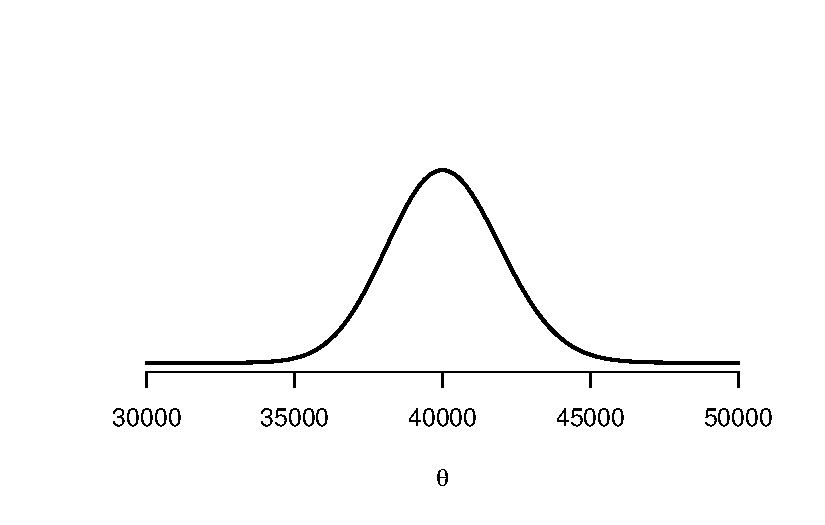
\includegraphics{intro_files/figure-pdf/fig-gammaElicitada-1.pdf}

}

\caption{\label{fig-gammaElicitada}Densidade a priori elicitada a partir
da média e do desvio padrão de informações passadas}

\end{figure}

É importante notar que a priori depende de um fator subjetivo. No
exemplo anterior, você poderia ter utilizado a moda e o desvio padrão
para fazer a sua elicitação, ou mesmo alguns quartis. Ou ainda,
utilizado uma Weibull ou outra distribuição contínua. Isto teria
resultado em prioris diferentes.

Naturalmente, isto nos conduziria a \textbf{posterioris} diferentes.
Esta é a principal crítica ao método bayesiano: duas pesquisas com a
mesma amostra podem ter resultados distintos, dependendo da priori.

Para evitar resultados discrepantes, temos que garantir que não haja
conflitos entre as fontes de informação. Em geral, vamos querer que a
\textbf{posteriori} esteja mas próxima da verossimilhança que da
\textbf{priori}.

\hypertarget{o-problema-da-exposiuxe7uxe3o}{%
\section{O problema da exposição}\label{o-problema-da-exposiuxe7uxe3o}}

Uma exposição gratuita recebeu vários visitantes em um dia. Nesta
exposição existe um livro de visitas, que o visitante pode optar por não
assinar. Os organizadores da exposição dizem que

\begin{itemize}
\tightlist
\item
  Entre 60\% e 80\% dos visitantes assinam o livro.
\item
  Em média, 100 pessoas visitam a exposição por dia.
\end{itemize}

Em um dia foram registrados 96 visitantes no livro. O que podemos dizer
sobre o número total de visitantes?

*Tente fazer um palpite sobre este total.**

Você provavelmente chegou em uma solução razoável, utilizando seus
conhecimentos matemáticos sobre grandezas proporcionais. Entretanto,
para fazer isto, você se utilizou de duas informações que não vieram da
amostra! A única informação proveniente da amostra é: 96 visitantes
assinaram o livro. Para dificultar um pouco mais, a amostra é de tamanho
1. Este é um exemplo típico no qual a a informação da \textbf{priori} é
relevante para fazer inferências.

\begin{solution}

Seja \(X\) o número de pessoas que assinaram o livro por dia. Seja
\(\tau\) o número de pessoas que visitam a exposição. Seja \(\theta\) a
probabilidade de um visitante qualquer assinar o livro. Neste primeiro
momento, assuma que \(\theta\) é uma constante igual a \(0,7\) (em outra
aula vamos trabalhar com \(\theta\) desconhecido)

O espaço paramétrico de \(\tau\) é \(T=\{0,1,2,\ldots\}\) * O
facilitador deve procurar uma distribuição que seja adequada para o
espaço \(T\). * Neste exemplo, escolheu-se trabalhar com
\(\tau\sim\hbox{Poisson}(a)\) * Lembrando que, em média (a priori) 100
pessoas visitam a exposição por dia, temos \[E[\tau]=a=100.\]

É natural supor que
\[f(x|\tau)={\tau \choose x}\left(\frac{7}{10}\right)^x \left(\frac{3}{10}\right)^{\tau-x},\;\; x=0,\ldots,\tau.\]
Como observamos \(x=96\), a verossimilhança será

\[\begin{align}
     L(\tau)=\left\{ \begin{array}{ll}{\tau \choose 96}\left(\frac{7}{10}\right)^{96}\left(\frac{3}{10}\right)^{\tau-96},& \;\; \tau\geq 96\\0,& cc \end{array}\right.
   \end{align}\]

Pelo Teorema de Bayes,

\[\begin{align}
   f(\tau|x)&=\frac{L(\tau)f(\tau)}{\sum_{t=0}^{\infty}L(t)f(t)}\\
   &=\frac{ {\tau \choose 96}\left(\frac{7}{10}\right)^{96} \left(\frac{3}{10}\right)^{\tau-96}\frac{e^{-100}{100}^\tau }{\tau!}}{\sum_{t=96}^{\infty}{t \choose 96}\left(\frac{7}{10}\right)^{96} \left(\frac{3}{10}\right)^{t-96}\frac{e^{-100} {100}^t }{t!}}\\
   &=\frac{{\tau \choose 96}\frac{30^\tau}{\tau!}}{\sum_{t=96}^{\infty}{t \choose 96}\frac{30^t}{t!}}=\frac{\frac{30^\tau}{(\tau-96)!}}{\sum_{t=96}^{\infty}\frac{30^t}{(t-96)!}}=\frac{e^{-30}30^{\tau-96}}{(\tau-96)!},
   \end{align}\]

para \(\tau=96,97,\ldots\). Mas, fazendo \(u=t-96\),

\[\begin{align}
\sum_{t=96}^{\infty}\frac{30^t}{(t-96)!}&=\sum_{u=0}^\infty \frac{30^{u+96}}{u!}=30^{96}\sum_{u=0}^\infty \frac{30^{u}}{u!}\\
&=30^{96}e^{30}\sum_{u=0}^\infty \frac{e^{-30}30^{u}}{u!}=30^{96}e^{30}
\end{align}\]

teremos, \[\begin{align}
f(\tau|x)&=\frac{e^{-30}30^{\tau-96}}{(\tau-96)!},
\end{align}\] para \(\tau=96,97,\ldots\).

Portanto, \(\tau|x\) tem distribuição
\[f(\tau|x)=\frac{e^{-30}30^{\tau-96}}{(\tau-96)!}.\] e \[\begin{align}
  E(\tau|x)&=\sum_{\tau=96}^{\infty}\tau\frac{e^{-30}30^{\tau-96}}{(\tau-96)!}=\sum_{u=0}^{\infty}(u+96)\frac{e^{-30}30^{u}}{u!}\\
&=\sum_{u=0}^{\infty}u\frac{e^{-30}30^{u}}{u!}+96\sum_{u=0}^{\infty}\frac{e^{-30}30^{u}}{u!}\\
&=30+96=126
  \end{align}\]

Uma estimativa para o número médio de pessoas que visitaram a exposição
naquele dia é \[E[\tau|x]=126.\]

\begin{Shaded}
\begin{Highlighting}[]
\FunctionTok{plot}\NormalTok{(}\DecValTok{96}\SpecialCharTok{:}\DecValTok{160}\NormalTok{,}\FunctionTok{dpois}\NormalTok{(}\DecValTok{96}\SpecialCharTok{:}\DecValTok{160} \SpecialCharTok{{-}} \DecValTok{96}\NormalTok{, }\DecValTok{30}\NormalTok{), }\AttributeTok{type=} \StringTok{\textquotesingle{}h\textquotesingle{}}\NormalTok{,}\AttributeTok{lwd =} \DecValTok{2}\NormalTok{, }\AttributeTok{xlab=}\StringTok{\textquotesingle{}\textquotesingle{}}\NormalTok{,}\AttributeTok{ylab=}\StringTok{\textquotesingle{}\textquotesingle{}}\NormalTok{)}

\FunctionTok{title}\NormalTok{( }\AttributeTok{xlab =} \FunctionTok{expression}\NormalTok{(tau), }\AttributeTok{ylab =} \StringTok{\textquotesingle{}Posteriori para tau\textquotesingle{}}\NormalTok{)}
\end{Highlighting}
\end{Shaded}

\begin{figure}[H]

{\centering 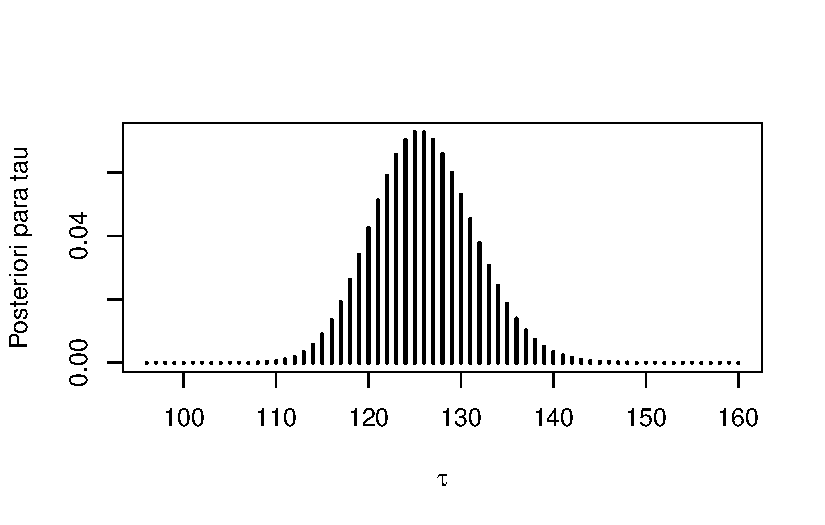
\includegraphics{intro_files/figure-pdf/fig-poissonExposicao1-1.pdf}

}

\caption{\label{fig-poissonExposicao1}Distribuição a posteriori para o
número de pessoas participaram da exposição.}

\end{figure}

\end{solution}

\emph{Resumo da aula 1}

\begin{itemize}
\item
  Existem duas fontes de informação na inferência bayesiana: os dados
  (verossimilhança) e a informação anterior (priori)
\item
  A informação \textbf{a priori} é subjetiva: pessoas diferentes tem
  prioris diferentes
\item
  O Teorema de Bayes combina as duas fontes em uma nova informação, dada
  pela distribuição \textit{a posteriori}
\item
  Os objetivos da inferência (estimação e testes) são feitos a partir da
  distribuição \textbf{a posteriori}
\end{itemize}

\bookmarksetup{startatroot}

\hypertarget{famuxedlias-conjugadas}{%
\chapter{Famílias conjugadas}\label{famuxedlias-conjugadas}}

\hypertarget{famuxedlia-de-distribuiuxe7uxf5es-conjugadas}{%
\section{Família de distribuições
conjugadas}\label{famuxedlia-de-distribuiuxe7uxf5es-conjugadas}}

Definição Dizemos que a priori \(f(\boldsymbol{\theta})\) é conjugada
para a verossimilhança \(L(\boldsymbol{\theta})\) se \emph{priori} e
\emph{posteriori} pertencem à mesma família de distribuições.

\begin{verbatim}
Sejam $X_1,\ldots,X_n$ variáveis aleatórias independentes com $X|\theta\sim \hbox{Bernoulli}(\theta)$ e $\theta\sim\hbox{Beta}(a,b)$. Então
\end{verbatim}

\[\begin{align}
    f(\theta|\boldsymbol{x})&\varpropto L(\theta)f(\theta) = \underbrace{\theta^{\sum_{i=1}^{n}x_i} (1-\theta)^{n-\sum_{i=1}^{n}x_i}}_{L(\theta)}\underbrace{\theta^{a-1}(1-\theta)^{b-1}}_{f(\theta)}\\
    &=\theta^{a+\sum_{i=1}^n x_i-1}(1-\theta)^{b+n-\sum_{i=1}^{n}x_i-1},
    \end{align}\]

logo
\(\theta|\boldsymbol{x}\sim\hbox{Beta}(a+\sum_{i=1}^{n}x_i,b+n-\sum_{i=1}^{n}x_i)\)
e a \emph{priori} beta é conjugada para a verossimilhança Bernoulli.

\hypertarget{conjugada-para-a-famuxedlia-exponencial}{%
\section{Conjugada para a família
exponencial}\label{conjugada-para-a-famuxedlia-exponencial}}

Famílias conjugadas são extremamente úteis tanto sob o ponto de vista
algébrico quando computacional. Entretanto, note que a definição de
família conjugada é ampla. Por exemplo, \emph{priori} e
\emph{posteriori} sempre pertence à grande família de todas as
distribuições de probabilidade, sendo esta a família conjugada trivial.

Famílias conjugadas não triviais são raras, existindo principalmente
quando a distribuição condicional dos dados pertence á família
exponencial.

Definição Considere que \(\Theta\) tem dimensão \(k\). Dizemos que
\(X|\boldsymbol{\theta}\) pertence à família exponencial (natural) se
\[f(x|\boldsymbol{\theta})=h(x)a(\boldsymbol{\theta})\exp\left\{\sum_{j=1}^k t_j(x)\theta_j\right\},\]
onde \(\mathcal{X}\) não depende de \(\boldsymbol{\theta}\). Além disso,
para a amostra (iid )\(X_1,\ldots,X_n|\boldsymbol{\theta}\),
\[f(\boldsymbol{x}|\boldsymbol{\theta})=h(\boldsymbol{x})a(\boldsymbol{\theta})^n\exp\left\{\sum_{j=1}^k T_j\theta_j\right\},\]
onde \(T_j=\sum_{i=1}^{n}t_j(x_i)\)

Se \(X|\boldsymbol{\theta}\) pertence à família exponencial, então
\[f(\boldsymbol{\theta})=c(\boldsymbol{r},s)a(\boldsymbol{\theta})^s\exp\left\{\sum_{j=1}^k r_j\theta_j\right\}\]
é uma \emph{priori} conjugada (ver O'Hagan (2005) para a existência
dessa distribuição). A \emph{posteriori} será dada por
\[f(\boldsymbol{\theta}|\boldsymbol{x})=c\left(\sum_{j=1}^k r_j+T_j,s+n\right)a(\boldsymbol{\theta})^{s+n}\exp\left\{\sum_{j=1}^k(r_j+T_j)\theta_j\right\}\]

Prova

\[\begin{align}
f(\boldsymbol{\theta}|\boldsymbol{x})&\varpropto \underbrace{a(\boldsymbol{\theta})^ne^{\sum_{j=1}^kT_j\theta_k}}_{L(\boldsymbol{\theta})}\underbrace{a(\boldsymbol{\theta})^s e^{\sum_{j=1}^k r_j\theta_k}}_{f(\boldsymbol{\theta})}\\
&a(\boldsymbol{\theta})^{n+s}e^{(\sum_{j=1}^{k}T_j+r_j)\theta_j}
\end{align}\]

Considere que \(\boldsymbol{\theta}\sim C(\boldsymbol{r},s)\) é a
distribuição conjugada da verossimilhança. Isto implica em
\(\boldsymbol{\theta}|\boldsymbol{x}\sim\hbox{C}(\boldsymbol{T}+\boldsymbol{r},s+n)\).
Note que a \emph{posteriori} atualiza a informação de \(s\) para \(s+n\)
e de \(r_j\) para \(T_j+r_j\). Logo, se imaginarmos que a priori é um
experimento hipotético, \(s\) seria o tamanho da amostra e
\(\boldsymbol{r}\) seriam as estatísticas suficientes deste modelo.

\hypertarget{conflito-entre-fontes-de-informauxe7uxe3o}{%
\section{Conflito entre fontes de
informação}\label{conflito-entre-fontes-de-informauxe7uxe3o}}

Considere que uma fábrica produz lotes de certos componentes
eletrônicos. O setor de qualidade faz inspeções periódicas através de
amostragem de 100 peças dentro de um lote. Todas as peças são testadas e
o número de falhas registrado. As últimas inspeções mostram que em torno
de 3\% das peças são defeituosas.

Uma nova amostra será selecionada. Sendo \(X\) o número de peças
defeituosas, uma verossimilhança adequada seria
\[\theta^x(1-\theta)^{100-x}\]

Sabemos que o modelo Beta\((r,s)\) é conjugado para esta
verossimilhança. Comparando a \emph{priori}
\[f(\theta)\varpropto \theta^{r-1}(1-\theta)^{s-1},\] com a
verossimilhança, podemos interpretar \(r\) como o número de componentes
defeituosos e \(s\)

Como temos as informações de vários lotes, podemos imaginar que um lote
hipotético de tamanho \(s=100\) foi selecionado e \(r=3\) peças
defeituosas foram encontradas.

Note que, com estes valores, a \emph{priori} exclui muitos valores do
espaço paramétrico, uma vez que \[\sqrt{Var(\theta)}=0,0167\] Se a
proporção amostral se manteve dentro dos 3\% não há problemas com isso.
Mas se ela aumentou (por causa de uma falha não detectada no processo),
como essa escolha vai influenciar nossa análise?

Para entender os efeitos da \emph{priori} sobre a \emph{posteriori},
vamos analisar dois cenários.

\begin{itemize}
\tightlist
\item
  Cenário 1: Foram encontradas 4 componentes defeituosos
\item
  Cenário 2: Foram encontrados 11 componentes defeituosos
\end{itemize}

\begin{figure}

{\centering 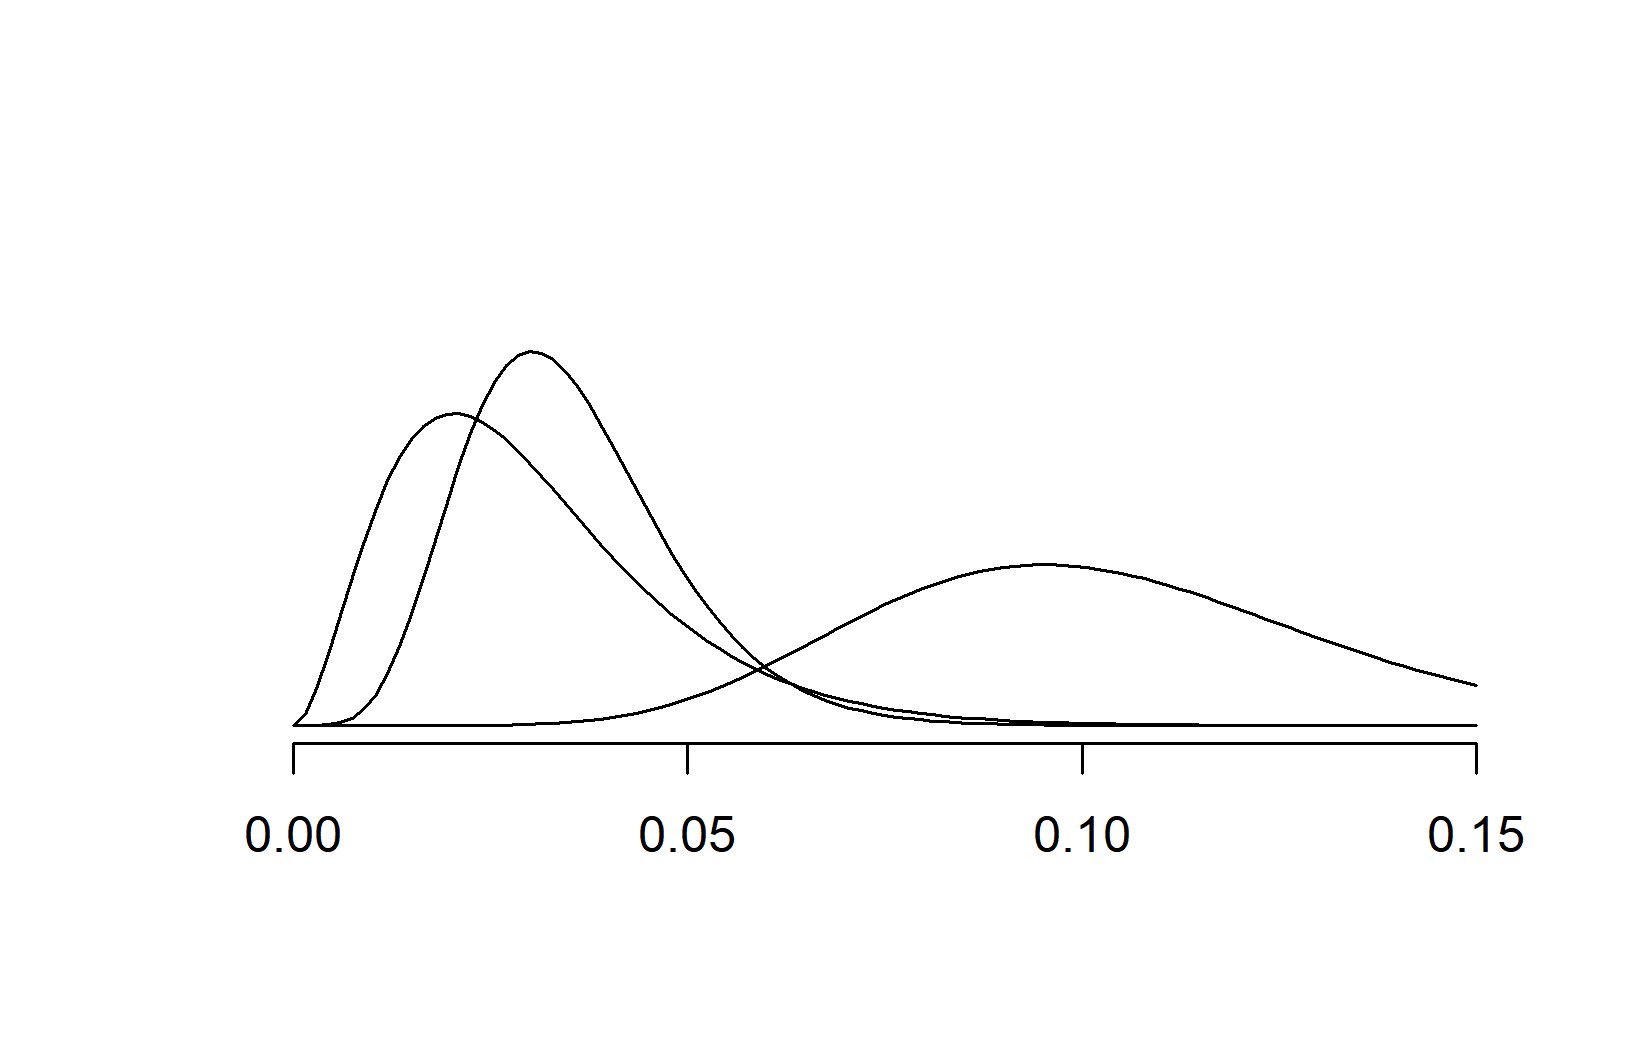
\includegraphics{conjugada_files/figure-pdf/conflito1-plot-1.png}

}

\caption{Figura 1. Cenário 1. Gráficos da verossimilhança, priori e
posteriori. \(E(\theta)\), \(\hat{\theta}\) e \(\tilde{\theta}\) são
média da priori, EMV e a média da posteriori..}

\end{figure}

\begin{figure}

{\centering 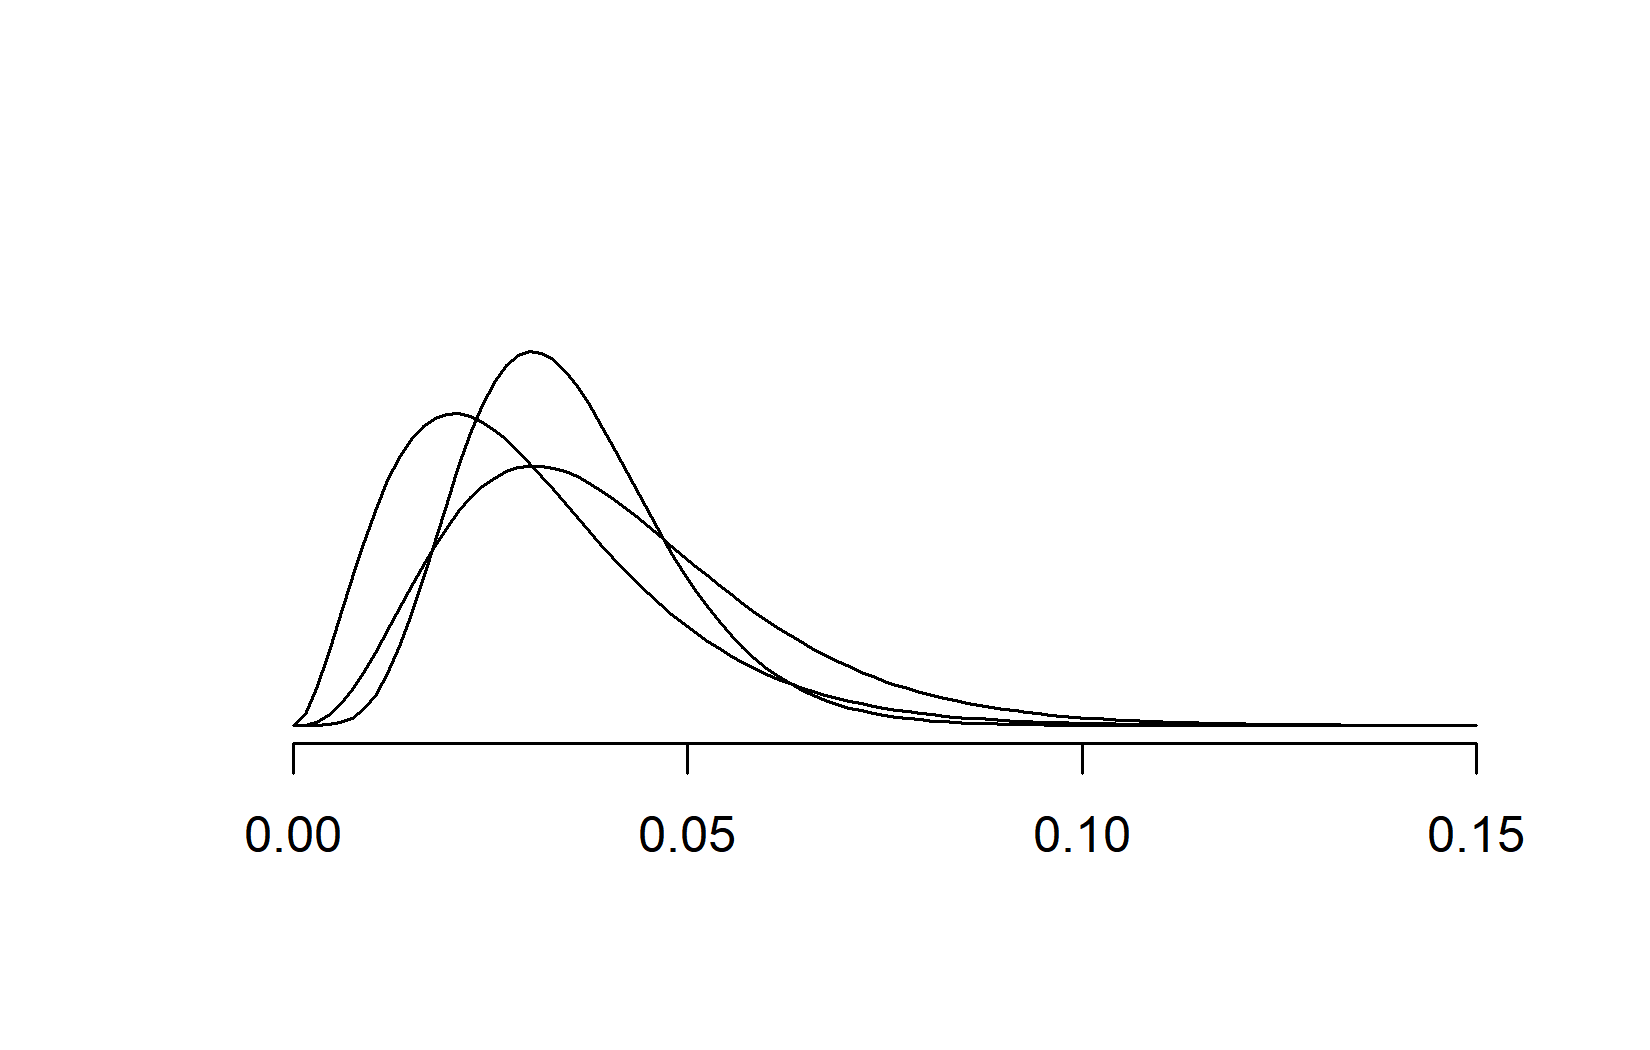
\includegraphics{conjugada_files/figure-pdf/conflito2-plot-1.png}

}

\caption{Figura 2. Cenário 2. Gráficos da verossimilhança, priori e
posteriori. \(E(\theta)\), \(\hat{\theta}\) e \(\tilde{\theta}\) são
média da priori, EMV e a média da posteriori..}

\end{figure}

Dizemos que há conflitos entre as fontes de informação quando a região
de maior densidade da \emph{posteriori} é pouco provável \emph{a priori}
e tem baixa verossimilhança. Isso aconteceu com o cenário 2. O motivo
para isso é que os dados geraram um valor atípico e a era muito
informativa (baixo desvio padrão), não tendo massa longe do suficiente
de \(E(\theta)\). Consideremos então a priori Beta(.3,9.7).

\[\begin{align}f(\mu,\phi|\boldsymbol{x})\propto f(x|\mu,\phi)f(\mu,\phi)\\
&\propto \phi^{\frac{n}{2}}e^{-\frac{\phi}{2}[ns^2 + n(\bar{x}-\mu)^2]}\times \phi^{\frac{1}{2}}e^{-\frac{\phi}{2C_0}(\mu-m_0)^2}\phi^{\frac{n_0}{2}-1}e^{-\frac{d_0}{2}\phi}\\
&= \phi^{\frac{1}{2}}e^{-\frac{\phi n}{2}(\bar{x}-\mu)^2 -\frac{\phi}{2C_0}(\mu-m_0)^2}\times \phi^{\frac{n+n_0}{2}-1}e^{-\frac{\phi}{2}\left(ns^2+d_0\right)}
\end{align}\]

\hypertarget{prioris-conjugadas-fora-da-famuxedlia-exponencial}{%
\section{Prioris conjugadas fora da família
exponencial}\label{prioris-conjugadas-fora-da-famuxedlia-exponencial}}

Famílias conjugadas fora da família exponencial são raras. Seja
\(X_1,\ldots,X_n\) variáveis aleatória independentes com
\(X_1|\phi,\psi\sim\hbox{Binomial Negativa}(\psi,\phi)\), onde

\[f(x|\phi,\psi)=\frac{\Gamma(x+\psi)}{\Gamma(\psi)x!}\phi^\psi (1-\phi)^x,\]
com \(\psi>0\), \(\phi\in(0,1)\) e \(x\in\mathbb{N}\). Se \(\psi\) é
conhecido, então
\[L(\boldsymbol{\theta})=\underbrace{\left[\frac{\prod_{i=1}^n\Gamma(x_i+\psi)}{\Gamma(\psi)^n\prod_{i=1}^n x_i!}\right]}_{h(\boldsymbol{x})}\underbrace{\phi^{n\psi}}_{a(\phi)}\exp\left\{ \underbrace{\sum_{i=1}^n x_i}_{t(\boldsymbol{x})} \underbrace{\log(1-\phi)}_{w(\phi)}\right\} \]

Então, \[\begin{align}
f(\phi|\psi)&=c(r,s)a(\phi)^s e^{rw(\phi)}\\
&=c(r,s)\phi^{s\psi}(1-\phi)^{r}
\end{align}\] é uma \(*priori*\) conjugada. Da expressão acima segue que
\(\phi|\psi \sim \hbox{Beta}(s\psi+1,r+1)\). A \(*posteriori*\)
(condicional) por sua vez é dada por
\[f(\phi|\boldsymbol{x},\psi)\varpropto \phi^{\psi(s+n)}(1-\phi)^{r+\sum_{i=1}^{n}x_i},\]
onde ainda
\(\phi|\psi,\boldsymbol{x}\sim\hbox{Beta}(\psi(s+n)+1,r+\sum_{i=1}^{n}x_i+1)\)
Note que para fazer a inferência completa, ainda necessitamos de
\(\psi|\boldsymbol{x}\), uma vez que
\[f(\phi,\psi|\boldsymbol{x})=f(\phi|\psi,\boldsymbol{x})f(\psi|\boldsymbol{x}).\]
Outro método de obter a conjunta \((\phi,\psi|\boldsymbol{x})\), sem a
necessidade de calcular \(\psi|\boldsymbol{x}\) será discutido na
próxima aula.

\bookmarksetup{startatroot}

\hypertarget{o-estimador-de-bayes}{%
\chapter{O estimador de bayes}\label{o-estimador-de-bayes}}

Considere o problema de tomar alguma decisão sobre \(\theta\) utilizando
uma estatística \(T(\mathbf{x})\).

Podemos determinar o quão ruim é a nossa decisão definindo uma função de
perda \(\mathcal{L}(\theta,T)\), com as seguintes características:

\begin{itemize}
\item
  \(\mathcal{L}(\theta,T)=0\) sempre que \(T\) for a decisão correta em
  relação à \(\theta\)
\item
  \(\mathcal{L}(\theta,T)>0\) em caso contrário.
\end{itemize}

Por exemplo, se \(T\) for um estimador para \(\theta\), a decisão
correta seria ter \(T=\theta\). Além disso, quanto mais afastado \(T\)
estiver de \(\theta\), pior é a decisão e maior deveria ser a perda.

No problema de estimação pontual, é usual utilizar a perda quadrática:
\[\mathcal{L}(\theta,T)=(T-\theta)^2,\] cujo esboço do gráfico é dado
abaixo:

\begin{Shaded}
\begin{Highlighting}[]
\FunctionTok{plot.new}\NormalTok{()}
\FunctionTok{plot.window}\NormalTok{(}\AttributeTok{xlim=}\FunctionTok{c}\NormalTok{(}\SpecialCharTok{{-}}\DecValTok{2}\NormalTok{,}\DecValTok{2}\NormalTok{), }\AttributeTok{ylim=}\FunctionTok{c}\NormalTok{(}\DecValTok{0}\NormalTok{,}\DecValTok{4}\NormalTok{))}
\FunctionTok{curve}\NormalTok{( x}\SpecialCharTok{\^{}}\DecValTok{2}\NormalTok{,}\SpecialCharTok{{-}}\DecValTok{2}\NormalTok{,}\DecValTok{2}\NormalTok{, }\AttributeTok{lwd =} \DecValTok{2}\NormalTok{, }\AttributeTok{add =}\NormalTok{ T)}
\FunctionTok{axis}\NormalTok{(}\DecValTok{1}\NormalTok{, }\AttributeTok{at =} \FunctionTok{c}\NormalTok{(}\SpecialCharTok{{-}}\DecValTok{2}\NormalTok{,}\SpecialCharTok{{-}}\DecValTok{1}\NormalTok{,}\DecValTok{0}\NormalTok{,}\DecValTok{1}\NormalTok{,}\DecValTok{2}\NormalTok{), }\AttributeTok{labels =} \FunctionTok{c}\NormalTok{(}\FunctionTok{expression}\NormalTok{(theta }\SpecialCharTok{{-}}\DecValTok{2}\NormalTok{),}\FunctionTok{expression}\NormalTok{(theta }\SpecialCharTok{{-}}\DecValTok{1}\NormalTok{),}\FunctionTok{expression}\NormalTok{(theta),}\FunctionTok{expression}\NormalTok{(theta }\SpecialCharTok{+}\DecValTok{1}\NormalTok{),}\FunctionTok{expression}\NormalTok{(theta }\SpecialCharTok{+}\DecValTok{2}\NormalTok{) ))}
\FunctionTok{axis}\NormalTok{(}\DecValTok{2}\NormalTok{)}
\FunctionTok{title}\NormalTok{( }\AttributeTok{ylab =} \StringTok{\textquotesingle{}Perda quadrática\textquotesingle{}}\NormalTok{,}\AttributeTok{xlab =} \StringTok{\textquotesingle{}T\textquotesingle{}}\NormalTok{)}
\end{Highlighting}
\end{Shaded}

\begin{figure}[H]

{\centering 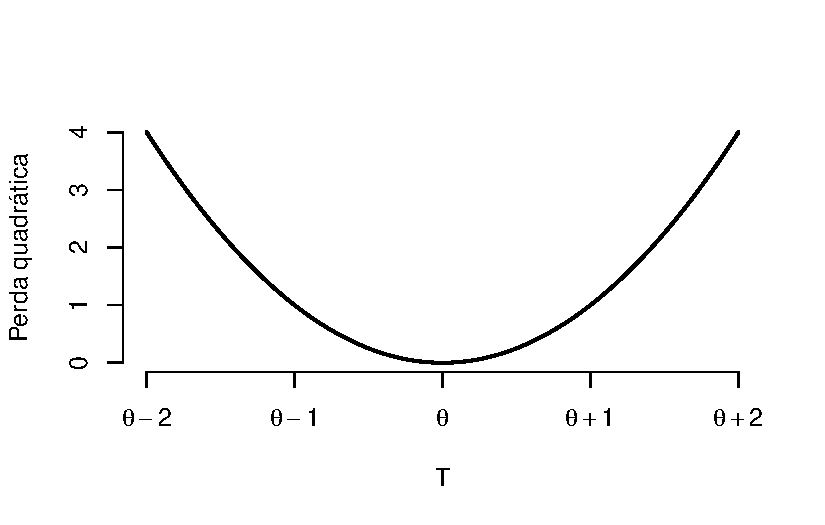
\includegraphics{estimacao_files/figure-pdf/unnamed-chunk-1-1.pdf}

}

\end{figure}

Para uma decisão \(T\) podemos calcular a perda média
\[R_T(\theta)=E(L(\theta,T))=\int L(\theta,T(\mathbf{x}))f(\mathbf{x}|\theta)d\mathbf{x}\]
A função acima é conhecida como risco da decisão \(T\) e é variável em
\(\theta\). Seu uso é simples: se \(R_T(\theta)<R_U(\theta)\), então em
média a decisão \(T\) tem menor perda que \(U\). Assim, a melhor escolha
entre as duas decisão é \(U\).

O risco associado à perda quadrática é denominado erro quadrático médio:

\[R_T(\theta)=E(T-\theta)^2= Var(T)+(E(T|\theta)-\theta)^2\] Ele possui
papel importante na inferência pontual frequentista, como por exemplo,
para definir o melhor estimador não viciado de variância uniformemente
mínima.

O risco de Bayes da decisão \(T\) é o valor esperado do seu respectivo
risco \textit{a priori}, \[r_T=\int R(\theta)f(\theta)d\theta,\] sendo
portanto uma constante. Qualquer decisão com o menor risco para todo
\(\theta\) também tem o menor risco de Bayes. Dizemos que \(T\) é o
estimador de Bayes se \(r_T<r_U\) para qualquer decisão \(U\).

Teorema

O estimador \(T\) que minimiza
\[\int \mathcal{L}(\theta,T(\mathbf{x}))f(\theta|\mathbf{x})d\theta\] é
o estimador de Bayes.

Exemplo

Vamos encontrar o estimador de Bayes para a perda quadrática. Temos que

\[\begin{align*}\int \mathcal{L}(\theta,T(\mathbf{x}))f(\theta|\mathbf{x})d\theta&=\int (T(\mathbf{x})-\theta)^2f(\theta|\mathbf{x})d\theta\\
    &=T(\mathbf{x})^2 +\int \theta^2f(\theta|\mathbf{x})d\theta-2T(\mathbf{x})\int \theta f(\theta|\mathbf{x})d\theta\\
    &= T(\mathbf{x})^2 + E(\theta^2|\mathbf{x}) -2T(\mathbf{x})E(\theta|\mathbf{x})\\
    &= T(\mathbf{x})^2 + E(\theta^2|\mathbf{x}) -2T(\mathbf{x})E(\theta|\mathbf{x}) \pm E(\theta|\mathbf{x})^2\\
    &=\left( T(\mathbf{x}) - E(\theta|\mathbf{x})\right)^2 +E(\theta^2|\mathbf{x})-E(\theta|\mathbf{x})^2\\
    &=\left( T(\mathbf{x}) - E(\theta|\mathbf{x})\right)^2 +Var(\theta|\mathbf{x})
\end{align*}\] A função acima é minimizada em
\(T(\mathbf{x})=E(\theta|\mathbf{x})\). Disto, mostra-se que
\[r_T\geq Var(\theta|\mathbf{x})\] e a variância da posteriori pode ser
utilizada como medida de erro. Como a unidade deste erro está ap
quadrado, é usual utilizarmos o desvio padrão da posteriori como medida
de erro.

\bookmarksetup{startatroot}

\hypertarget{o-modelo-normal}{%
\chapter{O modelo normal}\label{o-modelo-normal}}

\hypertarget{a-distribuiuxe7uxe3o-normal-gama}{%
\section{A distribuição
normal-gama}\label{a-distribuiuxe7uxe3o-normal-gama}}

Dizemos que \((X,Y)\sim NG(\mu,n_0,\nu,d^2)\) (lê-se normal-gama) se sua
função densidade conjunta é dada por

\[f(x,y)\propto y^{\frac{\nu+1}{2}-1}\exp\left\{-\frac{y}{2}n_0\left[(x-\mu)^2 + d^2\right]\right\}\]

onde \(\mu,x\in\mathbb{R}\) e \(d,y,c\in\mathbb{R}_+\). Colocando os
termos que não dependem de \(x\) junto com a constante de
proporcionalidade, podemos mostrar que

\[f(x|y)\propto \exp\left\{-\frac{y}{2}n_0(x-\mu)^2\right\}\] ou seja,
\(X|y\sim\hbox{Normal}(\mu,y^{-1}/n_0)\). Além disso, integrando
\(f(x,y)\) em \(x\), mostramos que

\[f(y)\propto y^{\frac{\nu+1}{2}-1}e^{-\frac{yn_0d^2}{2}}\int_{\mathbb{R}}\exp\left\{-\frac{y}{2}\left[n_0(x-\mu)^2\right]\right\}d\mu\propto y^{\frac{\nu}{2}-1}e^{-\frac{n_0d^2}{2}y}\]
ou seja, \(Y\sim\hbox{Gama}(\nu/2, n_0d^2/2)\). Por último, integrando
\(f(x,y)\) em \(y\) teremos

\[\begin{align}f(x)&\propto \int_0^\infty y^{\frac{\nu+1}{2}-1}\exp\left\{-\frac{y}{2}n_0\left[(x-\mu)^2 + d^2\right]\right\}dy \\&\propto \Gamma\left(\frac{\nu+1}{2}\right)\left\{1+\frac{\nu}{d^2}\frac{(x-\mu)^2}{\nu}\right\}^{-\frac{\nu+1}{2}}\end{align}\]
ou seja, \(X\sim t_{\nu}(\mu, d^2/\nu)\). Em especial, se \(\nu>1\)
então \(E(X)=\mu\) e, se \(\nu>2\) teremos que
\[Var(X)=\frac{d^2}{\nu-2}\]

\hypertarget{a-funuxe7uxe3o-de-verossimilhanuxe7a-1}{%
\section{A função de
verossimilhança}\label{a-funuxe7uxe3o-de-verossimilhanuxe7a-1}}

Seja \(X_1,\ldots,X_n\) uma amostra aleatória do modelo
\(X|\mu,\phi\sim\hbox{Normal}(\mu,\phi^{-1})\), onde \(\phi\),
denominado precisão, é o inverso da variância. A função de
verossimilhança deste modelo pode ser escrita como

\[L(\mu,\phi)\propto \phi^{\frac{n}{2}}\exp\left\{-\frac{n\phi}{2}(\bar{x}-\mu)^2 -\frac{ns^2\phi}{2}\right\}\]
onde \[s^2=\frac{1}{n}\sum_{i=1}^n(x_i-\bar{x})^2\] é a estimativa de
máxima verossimilhança para \(\phi^{-1}\).

\hypertarget{posteriori-com-prioris-impruxf3prias}{%
\section{Posteriori com prioris
impróprias}\label{posteriori-com-prioris-impruxf3prias}}

Considerando as prioris impróprias \(\pi(\phi)\propto \phi^{-1}\),
\(\pi(\mu)\propto 1\) e que \(\pi(\mu,\phi)=\pi(\mu)\pi(\phi)\), teremos
que

\[\pi(\mu,\phi|\boldsymbol{x})\propto \phi^{\frac{n}{2}-1}\left\{-\frac{\phi}{2}n\left[ (\bar{x}-\mu)^2 +s^2\right]\right\}\]
ou seja, \(\mu,\phi|\boldsymbol{x}\sim\hbox{NG}(\bar{x},n,n-1,s^2)\), o
que implica em:

\[\begin{align}
\mu|\phi,\boldsymbol{x}&\sim\hbox{Normal}\left(\bar{x},\frac{\phi^{-1}}{n}\right)\\
\phi|\boldsymbol{x}&\sim\hbox{Gama}\left(\frac{n-1}{2},\frac{ns^2}{2}\right)\\
\mu|\boldsymbol{x}&\sim t_{n-1}\left(\bar{x},\frac{s^2}{n-1}\right)
\end{align}\]

Disto, teremos que

\begin{longtable}[]{@{}lll@{}}
\toprule\noalign{}
Parâmetro & Estimativa & Erro \\
\midrule\noalign{}
\endhead
\bottomrule\noalign{}
\endlastfoot
\(\mu\) & \(\bar{x}\) & \(\frac{s}{\sqrt{n-3}}\) \\
\(\phi\) & \(\frac{n-1}{ns^2}\) & \(\frac{\sqrt{2(n-1)}}{s^2n}\) \\
\end{longtable}

\hypertarget{posteriori-com-a-priori-de-jeffreys}{%
\section{Posteriori com a priori de
Jeffreys}\label{posteriori-com-a-priori-de-jeffreys}}

O logaritmo da função de verossimilhança é

\[l(\mu,\phi)=\frac{n}{2}\log\phi -\frac{n}{2}\phi\left[(\bar{x}-\mu)^2 + s^2\right]\]

As derivadas de primeira ordem em \(\mu\) e \(\phi\) são \[\begin{align}
\frac{\partial}{\partial \mu}l(\mu,\phi)&=n\phi(\bar{x}-\mu)\\
\frac{\partial}{\partial \phi}l(\mu,\phi)&=\frac{n}{2\phi}-\frac{n}{2}\left[(\bar{x}-\mu)^2 + s^2\right]\\
\end{align}\]

e as de segunda ordem são \[\begin{align}
\frac{\partial^2}{\partial \mu^2}l(\mu,\phi)&=-n\phi\\
\frac{\partial^2}{\partial \phi^2}l(\mu,\phi)&=-\frac{n}{2\phi^2}\\
\frac{\partial^2}{\partial \mu\partial \phi}l(\mu,\phi)&=0\\
\end{align}
\] logo, a matriz de informação de Fisher é
\[\mathcal{I}_n(\mu,\phi)=n\left[\begin{array}{cc}\phi & 0 \\0 & \frac{1}{2\phi^2}\end{array}\right],\]
e a priori de Jeffreys é
\[\pi(\mu,\phi)\propto \sqrt{|\mathcal{I}_n(\mu,\phi)|}=\phi^{-1/2},\]
que implica na posteriori

\[\pi(\mu,\phi|\boldsymbol{x})\propto \phi^{\frac{n+1}{2}-1}\left\{-\frac{n\phi}{2}\left[(\bar{x}-\mu)^2 +s^2 \right]\right\}\]
ou seja, \(\mu,\phi|\boldsymbol{x}\sim\hbox{NG}(\bar{x},n,n,s^2)\), o
que implica em:

\[\begin{align}
\mu|\phi,\boldsymbol{x}&\sim\hbox{Normal}\left(\bar{x},\frac{\phi^{-1}}{n}\right)\\
\phi|\boldsymbol{x}&\sim\hbox{Gama}\left(\frac{n}{2},\frac{ns^2}{2}\right)\\
\mu|\boldsymbol{x}&\sim t_{n}\left(\bar{x},\frac{s^2}{n}\right)
\end{align}\]

Disto, teremos que

\begin{longtable}[]{@{}lll@{}}
\toprule\noalign{}
Parâmetro & Estimativa & Erro \\
\midrule\noalign{}
\endhead
\bottomrule\noalign{}
\endlastfoot
\(\mu\) & \(\bar{x}\) & \(\frac{s}{\sqrt{n-2}}\) \\
\(\phi\) & \(\frac{1}{s^{2}}\) & \(\frac{\sqrt{2}}{s^2\sqrt{n}}\) \\
\end{longtable}

\hypertarget{posteriori-para-a-priori-conjugada}{%
\section{Posteriori para a priori
conjugada}\label{posteriori-para-a-priori-conjugada}}

Considere que \((\mu,\phi)\sim \hbox{NG}(m_0,n_0,\nu_0,s^2_0)\). Esta
priori é conjugada para o modelo normal, uma vez que

\[\begin{align}
\pi(\mu,\phi|\boldsymbol{x})&\propto \phi^{\frac{n}{2}}\exp\left\{-\frac{\phi}{2}n\left[(\bar{x}-\mu)^2+ s^2\right]\right\}\phi^{\frac{\nu_0+1}{2}-1}\exp\left\{-\frac{\phi}{2}n_0\left[(\mu-m_0)^2 + s_0^2\right]\right\}\\
&\phi^{\frac{\nu_0+n}{2}-1}\exp\left\{-\frac{\phi}{2}\left[n(\bar{x}-\mu)^2 + n_0(\mu-m_0)^2+ns^2 + n_0s^2_0\right]\right\}\end{align}.\]
Como
\[n(\bar{x}-\mu)^2 +n_0(\mu-m_0)^2 = (n+n_0)(\mu-m_1)^2+\frac{n n_0}{n+n_0}(\bar{x}-m_0)^2\]
onde \[\begin{align}
m_1&=\frac{n}{n+n_0}\bar{x}+\frac{n_0}{n+n_0}m_0
\end{align},\] teremos \[\begin{align}
\pi(\mu,\phi|\boldsymbol{x})&\propto \phi^{\frac{\nu_1+1}{2}-1}\exp\left\{-\frac{\phi}{2}n_1\left[(\mu-m_1)^2 + d_1^2\right]\right\}\end{align},\]
onde \[\begin{align}
\nu_1&=\nu_0+n\\
n_1&=n_0+n\\
m_1&=\frac{n}{n1}\bar{x}+\frac{n_0}{n_1}m_0\\
d_1^2& = \frac{n_0n}{n_1^2}(\bar{x}-m_0)^2+\frac{n}{n_1}s^2 + \frac{n_0}{n_1}s^2_0
\end{align}\] ou seja,
\(\mu,\phi|\boldsymbol{x}\sim\hbox{NG}(m_1,n+n_0,\nu_0+n,d_1^2)\), o que
implica em:

\[\begin{align}
\mu|\phi,\boldsymbol{x}&\sim\hbox{Normal}\left(m_1,\frac{\phi^{-1}}{n+n_0}\right)\\
\phi|\boldsymbol{x}&\sim\hbox{Gama}\left(\frac{n+\nu_0}{2},\frac{(n+n_0)d_1^2}{2}\right)\\
\mu|\boldsymbol{x}&\sim t_{n}\left(m_1,\frac{d^2_1}{\nu_0+n}\right)
\end{align}\]

Disto, teremos que

\begin{longtable}[]{@{}
  >{\raggedright\arraybackslash}p{(\columnwidth - 4\tabcolsep) * \real{0.3472}}
  >{\raggedright\arraybackslash}p{(\columnwidth - 4\tabcolsep) * \real{0.4028}}
  >{\raggedright\arraybackslash}p{(\columnwidth - 4\tabcolsep) * \real{0.2500}}@{}}
\toprule\noalign{}
\begin{minipage}[b]{\linewidth}\raggedright
Parâmetro
\end{minipage} & \begin{minipage}[b]{\linewidth}\raggedright
Estimativa
\end{minipage} & \begin{minipage}[b]{\linewidth}\raggedright
Erro
\end{minipage} \\
\midrule\noalign{}
\endhead
\bottomrule\noalign{}
\endlastfoot
\(\mu\) & \(\frac{n}{n+n_0}\bar{x}+\frac{n_0}{n+n_0}m_0\) &
\(\frac{d_1}{\sqrt{n+\nu_0-2}}\) \\
\(\phi\) & \(\frac{n+\nu_0}{(n+n_0)d_1^2}\) &
\(\frac{\sqrt{2(n+\nu_0)}}{d_1^2(n+n_0)}\) \\
\end{longtable}

\hypertarget{detecuxe7uxe3o-de-outliers}{%
\section{Detecção de outliers}\label{detecuxe7uxe3o-de-outliers}}

\bookmarksetup{startatroot}

\hypertarget{binomial-negativa}{%
\chapter{Binomial negativa}\label{binomial-negativa}}

\hypertarget{o-modelo-binomial-negativo}{%
\section{O modelo binomial negativo}\label{o-modelo-binomial-negativo}}

A distribuição Poisson é muito comum em problemas de contagem. Como sua
esperança e variância são iguais, o termo sobredispersão foi cunhado na
literatura como uma variância maior que a média, o que seria indício de
que o modelo Poisson não é adequado (de modo análogo, há o conceito de
subdispersão, mas não é um fenômeno comum).

Dizemos que \(X|\rho,\phi\sim\hbox{Binomial Negativa}\) se

\[p(x|\rho,\phi)=\frac{\Gamma(\phi+x)}{x!\Gamma(\phi)}\rho^\phi(1-\rho)^x,\]
onde \(x\in\mathbb{N}\), \(\rho\in(0,1)\) e \(\phi>0\).

Existem diversos motivos para considerar o modelo binomial negativo uma
alternativa quando o modelo Poisson não parece ser adequado. Primeiro,
temos que \(E(X|\rho,\phi)=\phi(1-\rho)/\rho\) e
\(Var(X|\rho,\phi)=E(X|\rho,\phi)/\rho\), logo, a sobredispersão está
presente no modelo. Além disso, se
\(X|\lambda\sim\hbox{Poisson}(\lambda)\) e
\(\lambda\sim\hbox{Gama}(\phi, \rho/(1-\rho))\), então
\(X|\phi,\rho\sim\hbox{Binomial Negativa}(\phi,\rho)\) logo, este modelo
é uma mistura do modelo Poisson. Por último, fazendo
\[\mu=\phi\frac{1-\rho}{\rho}\Rightarrow \rho(\phi)=\frac{\phi}{\phi+\mu},\]
pode-de mostrar que
\[\lim_{\phi\rightarrow\infty}p(x|\phi)=\frac{e^{-\mu}\mu^x}{x!}\] ou
seja, o modelo Poisson também pode ser vist como um caso limite do
binomial negativo.

\hypertarget{priori-para-phi-condicionado}{%
\section{\texorpdfstring{Priori para \(\phi\)
condicionado}{Priori para \textbackslash phi condicionado}}\label{priori-para-phi-condicionado}}

Quando \(\phi\) é conhecido, a verossimilhança do modelo se torna

\[L(\rho|\phi)\propto \rho^{n\phi}(1-\rho)^{\sum_{i=1}^n x_i},\] logo, o
modelo Beta\((a,b)\) é conjugado, com a posteriori dada por
\[\rho|\boldsymbol{x},\phi\sim\hbox{Beta}\left(n\phi+a,\sum_{i=1}^n x_i+b\right).\]

A priori de Jeffreys é dada por

\[\pi(\rho)\propto \frac{1}{\rho(1-\rho)^{1/2}},\] o que implica na
posteriori
\[\rho|\boldsymbol{x},\phi\sim\hbox{Beta}\left(n\phi,\sum_{i=1}^n x_i+\frac{1}{2}\right).\]

\hypertarget{priori-para-phi}{%
\section{\texorpdfstring{Priori para
\(\phi\)}{Priori para \textbackslash phi}}\label{priori-para-phi}}

Seja \(\pi(\phi)\pi(\rho)\) a priori para \((\phi,\rho)\). Então,
teremos que

\[\pi(\phi,\rho|\boldsymbol{x})\propto \frac{\prod_{i=1}^n\Gamma(\phi+x_i)}{\Gamma(\phi)^n}\rho^{n\phi}(1-\rho)^{\sum_{i=1}^n x_i}\pi(\phi)\pi(\rho).\]

Assumindo qualquer uma das prioris da seção anterior, teremos

\[\pi(\phi,\rho|\boldsymbol{x})\propto \frac{\prod_{i=1}^n\Gamma(\phi+x_i)}{\Gamma(\phi)^n}B\left(a_0+n\phi,b_0+\sum_{i=1}^nx_i\right)\pi(\phi)\pi(\rho|\phi,\boldsymbol{x}),\]

logo,

\[\pi(\phi|\boldsymbol{x})\propto \frac{\prod_{i=1}^n\Gamma(\phi+x_i)}{\Gamma(\phi)^n}B\left(a_0+n\phi,b_0+\sum_{i=1}^nx_i\right)\pi(\phi)\]

Como a posteriori de \(\phi\) não é uma distribuição conhecida,
precisamos construir um simulador. O algoritmo Metropolis-Hastings é uma
boa escolha, uma vez que a constante de proporcionalidade da densidade é
desconhecida.

Algoritmo Metropolis-Hastings

O Metropolis-Hastings simula se utiliza de uma distribuição que sabemos
simular (denominada proposta) para gerar uma cadeia de Markov cuja
distribuição estacionária é a distribuição de interesse.

Na \(j\)-ésima itereção, a simulação do valor proposto \(\phi^*\) é
baseada no valor atual da cadeia, \(\phi^{(j-1)}\). Como \(\phi>0\), a
proposta \(\phi^*\sim \hbox{Gamma}(\tau\phi^{(j-1)},\tau)\) é adequada
uma vez que \[E(\phi^*)=\phi^{(j-1)}\] e
\[\sqrt{Var(\phi^*)}=\frac{\phi^{(j-1)}}{\tau}\] Acima, \(\tau\) é
denominado \emph{tunning} (afinação em tradução livre) e deve ser
escolhido para que a cadeia tenha o número de aceites da proposta
controlado (algo em torno de 23\% ).

Abaixo, segue o algoritmo

\begin{enumerate}
\def\labelenumi{\arabic{enumi}.}
\item
  Faça \(j=0\) e escolha um valor para \(\phi^{(0)}\) (a estimativa de
  máxima verossimilhança, por exemplo). Faça um contador de aceites,
  começando com \(k=0\).
\item
  Para o passo \(j\):
\end{enumerate}

\begin{itemize}
\tightlist
\item
  Simule \(\phi^*\sim\hbox{Gama}(\tau\phi^{j-1},\tau)\)
\item
  Calcule
\end{itemize}

\[prob = \frac{\pi(\phi^*|\boldsymbol{x})}{\pi(\phi^{(j-1)}|\boldsymbol{x})}\frac{g(\phi^{(j-1)}|\tau\phi^*,\tau)}{g(\phi^*|\tau\phi^{(j-1)},\tau)},\]
onde \(g(.|a,b)\) é a função densidade do modelo gama. + Simule
\(u\sim\hbox{Uniforme}(0,1)\). Se \(u<prob\), faça \(\phi^{(j)}=\phi^*\)
e \(k=k+1\) (houve um aceite). Senão, faça \(\phi^{(j)}=\phi^{(j-1)}\).

\bookmarksetup{startatroot}

\hypertarget{aproximauxe7uxe3o-normal-e-seu-uso-com-o-metropolis-hastings}{%
\chapter{Aproximação normal e seu uso com o
Metropolis-Hastings}\label{aproximauxe7uxe3o-normal-e-seu-uso-com-o-metropolis-hastings}}

\hypertarget{aproximauxe7uxe3o-da-posteriori-pela-distribuiuxe7uxe3o-normal}{%
\section{Aproximação da posteriori pela distribuição
normal}\label{aproximauxe7uxe3o-da-posteriori-pela-distribuiuxe7uxe3o-normal}}

Assuma que \(\boldsymbol{\theta}\in\mathbb{R}^q\). Seja
\(\ell(\boldsymbol{\theta})=\log L(\boldsymbol{\theta})\) a função
log-verossimilhança e \(\hat{\boldsymbol{\theta}}\) a estimativa de
máxima verossimilhaça para \(\boldsymbol{\theta}\). Considere a seguinte
aproximação de \(\ell(\boldsymbol{\theta})\) em séries de Taylor

\[\ell(\boldsymbol{\theta})\approx  \ell(\hat{\boldsymbol{\theta}})+\frac{1}{2}(\boldsymbol{\theta}-\hat{\boldsymbol{\theta}})'\mathcal{H}(\hat{\boldsymbol{\theta}})(\boldsymbol{\theta}-\hat{\boldsymbol{\theta}})\]
onde \(\boldsymbol{\theta}\) é a matriz hessiana (de derivadas segunda)
aplicada em \(\hat{\boldsymbol{\theta}}\). Deste modo, teremos que
\[\pi(\boldsymbol{\theta}|\boldsymbol{x})\propto \exp\left\{-\frac{1}{2}(\boldsymbol{\theta}-\hat{\boldsymbol{\theta}})'\left[-\mathcal{H}(\hat{\boldsymbol{\theta}})\right](\boldsymbol{\theta}-\hat{\boldsymbol{\theta}})\right\}\pi(\boldsymbol{\theta})\]

Utilizando a priori imprópria \(\pi(\boldsymbol{\theta})\), temos que
\(\boldsymbol{\theta}|\boldsymbol{x}\approx \hbox{Normal}(\hat{\boldsymbol{\theta}},-\mathcal{H}(\hat{\boldsymbol{\theta}})^{-1})\).

Note que as informações necessárias para a aproximação da posteriori
acima podem ser obtidas via função \texttt{optim}.

Exemplo A amostra abaixo foi simulada do modelo Gama\((\alpha,\beta)\)
(o valor dos parâmetros foram omitidos de propósito)

\begin{Shaded}
\begin{Highlighting}[]
\NormalTok{x}
\end{Highlighting}
\end{Shaded}

\begin{verbatim}
 [1] 0.2769550 1.1902521 1.1543901 0.6836040 1.2951363 0.8468467 0.7626888
 [8] 0.3830976 0.2270072 0.2785412 0.3853067 0.4818242 0.2021683 0.8914625
[15] 0.7718524 0.9455476 0.8702839 0.5309044 1.2858882 1.0415047
\end{verbatim}

Como \(\alpha,\beta>0\), considere que \(\alpha=\exp\{\theta_1\}\) e
\(\beta=\exp\{\theta_2\}\) (deste modo,
\(\boldsymbol{\theta}\in\mathbb{R}^2\)).

A função de log-verossimilhança deste modelo é

\begin{Shaded}
\begin{Highlighting}[]
\NormalTok{logveross }\OtherTok{\textless{}{-}} \ControlFlowTok{function}\NormalTok{(theta)\{ }\FunctionTok{sum}\NormalTok{(}\FunctionTok{dgamma}\NormalTok{(x, }\FunctionTok{exp}\NormalTok{(theta[}\DecValTok{1}\NormalTok{]), }\FunctionTok{exp}\NormalTok{(theta[}\DecValTok{2}\NormalTok{]), }\AttributeTok{log =}\NormalTok{ T))}
\NormalTok{\}}
\end{Highlighting}
\end{Shaded}

Podemos utilizar a função \texttt{optim} para obter as estimativas de
máxima verossimilhança e a matriz hessiana. Contudo, primeiro devemos
observar que esta função é um minimizador, logo, queremos que
\(\boldsymbol{\theta}\) que minimize \(-\ell({\boldsymbol{\theta}})\).

\begin{Shaded}
\begin{Highlighting}[]
\NormalTok{opt }\OtherTok{\textless{}{-}} \FunctionTok{optim}\NormalTok{( }\FunctionTok{c}\NormalTok{(}\DecValTok{0}\NormalTok{,}\DecValTok{0}\NormalTok{), }\ControlFlowTok{function}\NormalTok{(q) }\SpecialCharTok{{-}}\FunctionTok{logveross}\NormalTok{(q), }\AttributeTok{hessian =}\NormalTok{ T)}
\NormalTok{opt}
\end{Highlighting}
\end{Shaded}

\begin{verbatim}
$par
[1] 1.245897 1.567152

$value
[1] 7.435047

$counts
function gradient 
      65       NA 

$convergence
[1] 0

$message
NULL

$hessian
          [,1]      [,2]
[1,]  80.46195 -69.52104
[2,] -69.52104  69.52342
\end{verbatim}

No objeto \texttt{opt}, a lista \texttt{par} é o vetor com as
estimativas de máxima verossimilhança, enquanto que \texttt{hessian} é o
valor de \(-\mathcal{H}(\hat{\boldsymbol{\theta}})\).

A inversa de \texttt{opt\$hessian} vai dar a matriz de covariância entre
\(\theta_1\) e \(\theta_2\) a posteriori.

\begin{Shaded}
\begin{Highlighting}[]
\NormalTok{Sigma }\OtherTok{\textless{}{-}} \FunctionTok{solve}\NormalTok{(opt}\SpecialCharTok{$}\NormalTok{hessian)}
\NormalTok{Sigma}
\end{Highlighting}
\end{Shaded}

\begin{verbatim}
           [,1]       [,2]
[1,] 0.09138023 0.09137711
[2,] 0.09137711 0.10575762
\end{verbatim}

Agora, podemos simular \(\theta_1\) e \(\theta_2\) a posteriori:

\begin{Shaded}
\begin{Highlighting}[]
\FunctionTok{require}\NormalTok{(mvtnorm)}
\end{Highlighting}
\end{Shaded}

\begin{verbatim}
Carregando pacotes exigidos: mvtnorm
\end{verbatim}

\begin{Shaded}
\begin{Highlighting}[]
\NormalTok{theta\_sim }\OtherTok{\textless{}{-}} \FunctionTok{rmvnorm}\NormalTok{(}\DecValTok{500}\NormalTok{, opt}\SpecialCharTok{$}\NormalTok{par, Sigma)}
\end{Highlighting}
\end{Shaded}

Por último, podemos fazer inferências sobre \(\alpha=\exp\{\theta_1\}\)
e \(\beta=\exp\{\theta_2\}\):

\begin{Shaded}
\begin{Highlighting}[]
\CommentTok{\# intervalos de credibilidade para alfa}
\FunctionTok{quantile}\NormalTok{(}\FunctionTok{exp}\NormalTok{(theta\_sim[,}\DecValTok{1}\NormalTok{]), }\FunctionTok{c}\NormalTok{(.}\DecValTok{025}\NormalTok{,.}\DecValTok{975}\NormalTok{))}
\end{Highlighting}
\end{Shaded}

\begin{verbatim}
    2.5%    97.5% 
1.978850 6.350455 
\end{verbatim}

\begin{Shaded}
\begin{Highlighting}[]
\CommentTok{\# intervalos de credibilidade para beta}
\FunctionTok{quantile}\NormalTok{(}\FunctionTok{exp}\NormalTok{(theta\_sim[,}\DecValTok{2}\NormalTok{]), }\FunctionTok{c}\NormalTok{(.}\DecValTok{025}\NormalTok{,.}\DecValTok{975}\NormalTok{))}
\end{Highlighting}
\end{Shaded}

\begin{verbatim}
    2.5%    97.5% 
2.582863 8.865732 
\end{verbatim}

\hypertarget{metropolis-revisitado}{%
\section{Metropolis revisitado}\label{metropolis-revisitado}}

A diferença entre o algoritmo Metropolis e o Metropolis-Hastings está na
escolha da distribuição proposta. No primeiro, a proposta é simétrica,
\[g(x|y)=g(y|x).\] Com isso, teremos que
\[\frac{f(x)}{f(y)}\frac{g(y|x)}{g(x|y)}=\frac{f(x)}{f(y)}\] e a
probabilidade de aceitação da cadeia é baseada somente na distribuição
alvo \(f\).

No algoritmo Metropolis, é comum escolher a distribuição proposta como
sendo uma normal. Uma escolha razoável é utilizar como proposta
aproximação normal vista na seção anterior.

Exemplo Consideremos novamente a amostra do exemplo anterior. A função
de verossimilhança é
\[L(\theta)=\prod_{i=1}^n \frac{\beta(\theta_2)^{\alpha(\theta_1)}}{\Gamma(\alpha(\theta_1))} x_i^{\alpha(\theta_1)-1}e^{-\beta(\theta_2)x_i}\]
onde \(\alpha(\theta_1)=e^{\theta_1}\),
\(\beta(\theta_2)=e^{\theta_2}\). Além disso ,considere ad prioris
independentes \(\theta_i\sim\hbox{Normal}(0,100)\). Então, devemos
simular do modelo

\[\pi(\theta|\boldsymbol{x})\propto \left[\frac{\beta(\theta_2)^{\alpha(\theta_1)}}{\Gamma(\alpha(\theta_1))}\right]^n \left[\prod_{i=1}^n x_i\right]^{\alpha(\theta_1)}e^{-\beta(\theta_2)\sum_{i=1}^{n}x_i}e^{-\frac{1}{200}(\theta_1^2 + \theta_2^2)}\]

A posteriori aproximada, que encontramos no exemplo anterior é
\[\boldsymbol{\theta}|\boldsymbol{x}\approx N \left[ \left(\begin{array}{c}1,24\\1,56 \end{array}\right),\left(\begin{array}{cc}0,09 & 0,09\\0,09 &0,11\end{array}\right)\right]\]

Vamos aproveitar a estrutura de covariâncias acima para usar a proposta

\[\boldsymbol{\theta}^*|\boldsymbol{x}\sim N \left[ \boldsymbol{\theta}^{(j-1)},\tau\left(\begin{array}{cc}0,09 & 0,09\\0,09 &0,11\end{array}\right)\right]\]
onde \(\boldsymbol{\theta}^*\) é o candidato gerado e
\(\boldsymbol{\theta}^{(j)}\) é o estado atual da cadeia e \(\tau\) é o
\textbf{tunning} da cadeia.

\begin{Shaded}
\begin{Highlighting}[]
\NormalTok{B }\OtherTok{\textless{}{-}} \DecValTok{10000} \CommentTok{\# número de iterações}
\NormalTok{theta }\OtherTok{\textless{}{-}} \FunctionTok{array}\NormalTok{(}\ConstantTok{NA\_real\_}\NormalTok{, }\FunctionTok{c}\NormalTok{(B,}\DecValTok{2}\NormalTok{))}

\NormalTok{theta[}\DecValTok{1}\NormalTok{,] }\OtherTok{\textless{}{-}}\NormalTok{ opt}\SpecialCharTok{$}\NormalTok{par }\CommentTok{\# valor inicial da cadeia é a emv}
\NormalTok{tau }\OtherTok{\textless{}{-}} \DecValTok{1}             \CommentTok{\# tunning}
\NormalTok{cont }\OtherTok{\textless{}{-}} \DecValTok{0}            \CommentTok{\# contador de aceites}

\ControlFlowTok{for}\NormalTok{(j }\ControlFlowTok{in} \DecValTok{2}\SpecialCharTok{:}\NormalTok{B)\{}
  \CommentTok{\#simule um candidato}
\NormalTok{  theta\_cand }\OtherTok{\textless{}{-}} \FunctionTok{rmvnorm}\NormalTok{(}\DecValTok{1}\NormalTok{, theta[j}\DecValTok{{-}1}\NormalTok{,], tau}\SpecialCharTok{*}\NormalTok{Sigma)}
  
  \CommentTok{\# calcule a probabilidade do salto}
\NormalTok{  lnum }\OtherTok{\textless{}{-}} \FunctionTok{logveross}\NormalTok{(theta\_cand) }\SpecialCharTok{+}
    \FunctionTok{sum}\NormalTok{(}\FunctionTok{dnorm}\NormalTok{(theta\_cand[}\DecValTok{1}\NormalTok{,],}\DecValTok{0}\NormalTok{,}\DecValTok{10}\NormalTok{, }\AttributeTok{log =}\NormalTok{ T))}
  
\NormalTok{  lden }\OtherTok{\textless{}{-}} \FunctionTok{logveross}\NormalTok{(theta[j}\DecValTok{{-}1}\NormalTok{,]) }\SpecialCharTok{+}
    \FunctionTok{sum}\NormalTok{(}\FunctionTok{dnorm}\NormalTok{(theta[j}\DecValTok{{-}1}\NormalTok{,],}\DecValTok{0}\NormalTok{,}\DecValTok{10}\NormalTok{, }\AttributeTok{log =}\NormalTok{ T))}
  
\NormalTok{  prob }\OtherTok{\textless{}{-}} \FunctionTok{exp}\NormalTok{( lnum }\SpecialCharTok{{-}}\NormalTok{ lden)}
  
  \CommentTok{\# verifique o salto}
\NormalTok{  u }\OtherTok{\textless{}{-}} \FunctionTok{runif}\NormalTok{(}\DecValTok{1}\NormalTok{)}
  \ControlFlowTok{if}\NormalTok{( u }\SpecialCharTok{\textless{}}\NormalTok{ prob)\{}
\NormalTok{    theta[j, ] }\OtherTok{\textless{}{-}}\NormalTok{ theta\_cand}
\NormalTok{    cont }\OtherTok{\textless{}{-}}\NormalTok{ cont}\SpecialCharTok{+}\DecValTok{1}
\NormalTok{  \} }\ControlFlowTok{else}\NormalTok{ \{}
\NormalTok{    theta[j,] }\OtherTok{\textless{}{-}}\NormalTok{ theta[j}\DecValTok{{-}1}\NormalTok{,]}
\NormalTok{  \}}
\NormalTok{\}}

\NormalTok{cont}\SpecialCharTok{/}\NormalTok{B}
\end{Highlighting}
\end{Shaded}

\begin{verbatim}
[1] 0.5628
\end{verbatim}

\begin{Shaded}
\begin{Highlighting}[]
\NormalTok{theta\_sim }\OtherTok{\textless{}{-}}\NormalTok{ theta[ }\FunctionTok{seq}\NormalTok{(B}\SpecialCharTok{/}\DecValTok{2}\NormalTok{, B, }\DecValTok{15}\NormalTok{),]}
\FunctionTok{acf}\NormalTok{(theta\_sim)}
\end{Highlighting}
\end{Shaded}

\begin{figure}[H]

{\centering 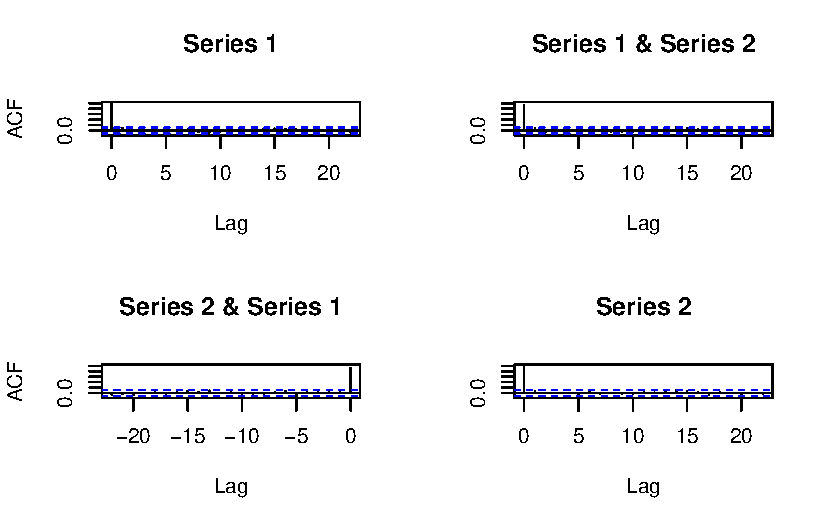
\includegraphics{aproximacaoNormal_files/figure-pdf/unnamed-chunk-8-1.pdf}

}

\end{figure}

Por fim, as estimativas intervalares para \((\alpha,\beta)\) são

\begin{Shaded}
\begin{Highlighting}[]
\FunctionTok{quantile}\NormalTok{(}\FunctionTok{exp}\NormalTok{(theta\_sim[,}\DecValTok{1}\NormalTok{]), }\FunctionTok{c}\NormalTok{(.}\DecValTok{025}\NormalTok{,.}\DecValTok{975}\NormalTok{))}
\end{Highlighting}
\end{Shaded}

\begin{verbatim}
    2.5%    97.5% 
1.699256 5.644593 
\end{verbatim}

\begin{Shaded}
\begin{Highlighting}[]
\CommentTok{\# intervalos de credibilidade para beta}
\FunctionTok{quantile}\NormalTok{(}\FunctionTok{exp}\NormalTok{(theta\_sim[,}\DecValTok{2}\NormalTok{]), }\FunctionTok{c}\NormalTok{(.}\DecValTok{025}\NormalTok{,.}\DecValTok{975}\NormalTok{))}
\end{Highlighting}
\end{Shaded}

\begin{verbatim}
    2.5%    97.5% 
2.087772 7.675778 
\end{verbatim}

\bookmarksetup{startatroot}

\hypertarget{misturas-de-distribuiuxe7uxf5es}{%
\chapter{Misturas de
distribuições}\label{misturas-de-distribuiuxe7uxf5es}}

Dizemos que \(X\sim f(.)\) é uma mistura se existe uma variável \(Z\)
tal que

\[f(x)=\int f(x|z)f(z)dz.\]

A variável \(Z\) é denominada latente e a função \(f(x,z)\) é denominada
modelo aumentado.

Seja \((X_1,Z_1),\ldots,(X_n,Y_n)\) uma amostra aleatória do modelo
aumentado \(f(x,z|\theta)\) e seja \(\pi(\theta)\) a priori para
\(\theta\). Existem situações nas quais é mais fácil simular do modelo
\[\pi(\theta,\boldsymbol{z}|\boldsymbol{x})\varpropto f(\boldsymbol{x},\boldsymbol{z}|\theta)\pi(\theta).\]

A distribuição de \(\theta\) (ou \(\boldsymbol{Z}\)) dado as demais
variáveis do modelo é denominada condicional completa, que neste
problema são:

\[f(\boldsymbol{z}|\boldsymbol{x},\theta)\] e
\[\pi(\theta|\boldsymbol{z},\boldsymbol{x},\theta)\]

Em particular, se é fácil simular das condicionais completas, podemos
utilizar o Amostrador de Gibbs, que consiste no seguinte algoritmo:

Amostrador de Gibbs

Inicie a cadeia com fazendo \(j=0\) e escolhendo \(\theta^{(0)}\)

No \(j\)-ésimo passo:

\begin{enumerate}
\def\labelenumi{\arabic{enumi}.}
\item
  Simule
  \(\boldsymbol{z^{(j)}}\sim f(\boldsymbol{z}|\boldsymbol{x},\theta^{(j-1)})\)
\item
  Simule \(\theta^{(j)}\sim \pi(\theta|\boldsymbol{z},\boldsymbol{x})\)
\end{enumerate}

O Amostrador de Gibbs é uma cadeia de Markov cuja distribuição
estacionária é \(\pi(\theta,\boldsymbol{z}|\boldsymbol{x})\)

\hypertarget{modelos-com-inflauxe7uxe3o-de-zeros}{%
\section{Modelos com inflação de
zeros}\label{modelos-com-inflauxe7uxe3o-de-zeros}}

Quando são observados mais zeros do que o esperado pelo modelo de
contagem assumido para a verossimilhança, é usual considerar um modelo
com inflação de zeros. Nesse tipo de modelo, assumimos que existe uma
variável \(Z|p\sim\hbox{Bernoulli}(\rho)\) tal que:

\[X=\left\{\begin{array}{ll}0, & \hbox{se }Z=1\ \\ Y,&\hbox{se }Z=0\end{array}\right.\]
onde \(Y\sim h(.|\theta)\) é o modelo de contagem. Apenas \(X\) é
observado e, como

\[\begin{align}P(X=0|\theta,p)&=P(X=0|Z=0,\theta)P(Z=0|\rho)+P(X=0|Z=1,\theta)P(Z=1|\rho)\\&=(1-\rho)h(0|\theta)+\rho\end{align}\]
a probabilidade de observar um zero está entre \(h(0|\theta)\) e 1, o
que caracteriza a inflação.

Agora, considere um modelo inflacionado de zeros aumentado:

\[f(x,z|\theta,\rho)=f(x|z,\theta)f(z|\rho)=f(x|z,\theta)\rho^z(1-\rho)^{1-z}.\]
Note que

\[f(x|z,\theta)=\left\{
\begin{array}{ll}
h(x|\theta),&\hbox{ se }z=0,\\
I(x=0),&\hbox{ se }z=1\\
\end{array}\right.\] logo, a distribuição conjunta
\(f(x,z|\theta,\rho)\) é dada por

\[\begin{array}{c|cc}\hline & x=0 & \hbox{qualquer }x> 0 \\ \hline
z=0 & h(0|\theta)(1-\rho) & h(x|\theta)(1-\rho) \\
z=1 & \rho & 0 \\ \hline
\end{array}
\] Então,

\[\begin{align}
\prod_{i=1}^n f(x_i,z_i|\theta,\rho)&=\prod_{i=1}^n [h(0|\theta)(1-\rho)]^{I(x_i=0,z_i=0)}[h(x_i|\theta)(1-\rho)]^{I(x_i>0,z_i=0)}\rho^{I(x_i=0,z_i=1)}\\
&=\prod_{i=1}^n [h(x_i|\theta)(1-\rho)]^{I(z_i=0)}\rho^{I(x_i=0,z_i=1)}\\
&=\prod_{i=1}^n(1-\rho)^{I(z_i=0)}\rho^{I(x_i=0,z_i=1)}\prod_{i=1}^n [h(x_i|\theta)]^{I(z_i=0)}\end{align}\]
e, notando que \(I(z_i=0)=1-z_i,\)

\[\begin{align}
\prod_{i=1}^n f(x_i,z_i|\theta,\rho)&=
(1-\rho)^{n-\sum_{i=1}^n z_i}\rho^{\sum_{i=1}^n z_iI(x_i=0)}\prod_{i=1}^n [h(x_i|\theta)]^{1-z_i}\end{align}\]

Considere, a priori, que \(\theta\) e \(\rho\) são independentes. Seja
\(\pi(\theta)\) a priori para \(\theta\) e considere que
\(\rho\sim\hbox{Beta}(a,b)\). Então, as condicionais completas para
\(\theta\) e \(\rho\) são

\[\begin{align}
\pi(\theta|\rho,\boldsymbol{z},\boldsymbol{x})&\propto \prod_{i=1}^n h(x_i|\theta)^{1-z_i}\pi(\theta),\\
\pi(\rho|\theta,\boldsymbol{z},\boldsymbol{x})&\propto \rho^{\sum_{i=1}^n z_iI(x_i=0)+a-1}(1-\rho)^{n-\sum_{i=1}^n z_i+b-1},\\
\end{align}\]

Para a condicional completa de \(z_i\), notemos que
\[P(Z_i=1|x_i>0)=\frac{P(Z_i=1,X_i>0)}{P(X_i>0)}=0,\] e que

\[P(Z_i=z|x_i=0)= \left\{\begin{array}{ll}\frac{P(Z_i=0,X_i=0)}{P(X_i=0)}=\frac{h(0|\theta)(1-\rho)}{\rho+(1-\rho)h(0|\theta)},&,z=0\\
\frac{P(Z_i=1,X_i=0)}{P(X_i=0)}=\frac{\rho}{\rho+(1-\rho)h(0|\theta)},&z=1\end{array}\right.,\]
logo
\[\pi(z_i|\theta,\rho,\boldsymbol{x},\boldsymbol{z}_{(-i)})=\left\{\begin{array}{ll}\hbox{Bernoulli}\left( \frac{\rho}{\rho+(1-\rho)h(0|\theta)}\right),&\hbox{ se }x_i=0\\
I(z_i=0),&\hbox{ se } x_i>0\\ \end{array}\right.\]

Portanto, um amostrador de Gibbs para um modelo inflacionado de zeros é

Amostrador de Gibbs para o modelo inflado de zeros

Faça \(j=0\) e dê os valores iniciais \(\theta^{(0)}\) e \(\rho^{(0)}\).

No \(j\)-ésimo passo:

\begin{enumerate}
\def\labelenumi{\arabic{enumi}.}
\item
  Para \(i\in\{1,\ldots,n\}\), se \(x_i>0\) faça \(z_i=0\). Senão,
  simule
  \[z_i^{(j)}\sim \hbox{Bernoulli}\left(\frac{\rho^{(j-1)}}{\rho^{(j-1)}+(1-\rho^{(j-1)})h(x_i|\theta^{(j-1)})}\right)\]
\item
  Simule
  \(\rho^{(j)}\sim\hbox{Beta}(a+\sum_{i=1}^n z_i^{(j)}I(x_i=0),b+n-\sum_{i=1}^n z_i^{(j)})\)
\item
  Simule \(\theta^{(j)}\) de
  \[\pi(\theta|\rho^{(j)},\boldsymbol{z}^{(j)},\boldsymbol{x})\propto \prod_{i=1}^n h(x_i|\theta^{(j)})^{1-z_i^{(j)}}\pi(\theta^{(j)}).\]
\end{enumerate}

Exemplo - A Poisson inflada de zeros

Neste exemplo, vamos considerar que a distribuição da contagem é
Poisson(\(\theta\)) e que \(\theta\sim\hbox{Gama}(r,s)\). Então,

\[\begin{align}
\pi(\theta|\rho^{(j)},\boldsymbol{z}^{(j)},\boldsymbol{x})&\propto \prod_{i=1}^{n} h(x_{i} | \theta )^{ 1-z_{i}^{(j)} }\pi(\theta)= 
 \prod_{i=1}^{n} \left[\frac{ e^{-\theta}\theta^{x_i} }{x_i!}\right]^{1-z_{i}^{(j)}}\frac{s^r}{\Gamma(r)}\theta^{r-1} e^{-s\theta}\\&\propto \theta^{\sum_{i=1}^n x_i(1-z_i^{(j)})+r-1}e^{-(n-\sum_{i=1}^n z_i^{(j)}+s)\theta}
 \end{align},\]

ou seja,
\(\theta^{(j)}|\rho^{(j)},\boldsymbol{z}^{(j)},\boldsymbol{x}\sim\hbox{Gama}(\sum_{i=1}^n x_i(1-z_i^{(j)})+r,n-\sum_{i=1}^n z_i^{(j)}+s)\)

Os dados abaixo representam o número anual de furacões atlânticos
grandes (categoria 4 ou 5) entre 1987 e 2012, nos Estados Unidos.

\begin{Shaded}
\begin{Highlighting}[]
\NormalTok{fur }\OtherTok{\textless{}{-}}  \FunctionTok{c}\NormalTok{(}\DecValTok{0}\NormalTok{, }\DecValTok{0}\NormalTok{ ,}\DecValTok{1}\NormalTok{,}
\DecValTok{0}\NormalTok{, }\DecValTok{0}\NormalTok{, }\DecValTok{1}\NormalTok{, }\DecValTok{0}\NormalTok{, }\DecValTok{0}\NormalTok{, }\DecValTok{1}\NormalTok{, }\DecValTok{0}\NormalTok{, }\DecValTok{0}\NormalTok{, }\DecValTok{2}\NormalTok{, }\DecValTok{2}\NormalTok{,}
\DecValTok{0}\NormalTok{, }\DecValTok{0}\NormalTok{, }\DecValTok{1}\NormalTok{, }\DecValTok{1}\NormalTok{, }\DecValTok{3}\NormalTok{, }\DecValTok{4}\NormalTok{, }\DecValTok{0}\NormalTok{, }\DecValTok{0}\NormalTok{, }\DecValTok{2}\NormalTok{, }\DecValTok{0}\NormalTok{,}
\DecValTok{0}\NormalTok{, }\DecValTok{0}\NormalTok{, }\DecValTok{0}\NormalTok{)}
\end{Highlighting}
\end{Shaded}

A frequência relativa de zeros é 0,58. Considerando o modelo
Poisson\((\theta)\) com \(\pi(\theta)\propto \theta^{-1}\), temos que

\begin{Shaded}
\begin{Highlighting}[]
\NormalTok{r1 }\OtherTok{\textless{}{-}} \FunctionTok{sum}\NormalTok{(fur)}
\NormalTok{s1 }\OtherTok{\textless{}{-}} \FunctionTok{length}\NormalTok{(fur)}
\FunctionTok{plot}\NormalTok{(}\FunctionTok{table}\NormalTok{(fur)}\SpecialCharTok{/}\NormalTok{s1, }\AttributeTok{type=} \StringTok{\textquotesingle{}p\textquotesingle{}}\NormalTok{, }\AttributeTok{xlab=}\StringTok{\textquotesingle{}No. anual de mortes pod fur\textquotesingle{}}\NormalTok{, }\AttributeTok{ylab =} \StringTok{\textquotesingle{}Probabilidade\textquotesingle{}}\NormalTok{, }\AttributeTok{col =} \StringTok{\textquotesingle{}cyan3\textquotesingle{}}\NormalTok{, }\AttributeTok{pch=}\DecValTok{16}\NormalTok{)}
\FunctionTok{lines}\NormalTok{(}\DecValTok{0}\SpecialCharTok{:}\DecValTok{4}\NormalTok{,}\FunctionTok{table}\NormalTok{(fur)}\SpecialCharTok{/}\NormalTok{s1, }\AttributeTok{col =} \StringTok{\textquotesingle{}cyan3\textquotesingle{}}\NormalTok{)}
\FunctionTok{points}\NormalTok{(}\DecValTok{0}\SpecialCharTok{:}\DecValTok{4}\NormalTok{, }\FunctionTok{dnbinom}\NormalTok{(}\DecValTok{0}\SpecialCharTok{:}\DecValTok{4}\NormalTok{, }\AttributeTok{size =}\NormalTok{ r1, }\AttributeTok{prob =}\NormalTok{ s1}\SpecialCharTok{/}\NormalTok{(}\DecValTok{1}\SpecialCharTok{+}\NormalTok{s1)), }\AttributeTok{pch=}\DecValTok{16}\NormalTok{, }\AttributeTok{col =} \StringTok{\textquotesingle{}brown\textquotesingle{}}\NormalTok{)}
\FunctionTok{lines}\NormalTok{(}\DecValTok{0}\SpecialCharTok{:}\DecValTok{4}\NormalTok{, }\FunctionTok{dnbinom}\NormalTok{(}\DecValTok{0}\SpecialCharTok{:}\DecValTok{4}\NormalTok{, }\AttributeTok{size =}\NormalTok{ r1, }\AttributeTok{prob =}\NormalTok{ s1}\SpecialCharTok{/}\NormalTok{(}\DecValTok{1}\SpecialCharTok{+}\NormalTok{s1)), }\AttributeTok{col =} \StringTok{\textquotesingle{}brown\textquotesingle{}}\NormalTok{)}

\FunctionTok{legend}\NormalTok{(}\StringTok{\textquotesingle{}bottomleft\textquotesingle{}}\NormalTok{,}\FunctionTok{c}\NormalTok{(}\StringTok{\textquotesingle{}Freq. relativa\textquotesingle{}}\NormalTok{,}\StringTok{\textquotesingle{}Pred. post. Poisson\textquotesingle{}}\NormalTok{), }\AttributeTok{fill=}\FunctionTok{c}\NormalTok{(}\StringTok{\textquotesingle{}cyan3\textquotesingle{}}\NormalTok{,}\StringTok{\textquotesingle{}brown\textquotesingle{}}\NormalTok{), }\AttributeTok{bty=}\StringTok{\textquotesingle{}n\textquotesingle{}}\NormalTok{)}
\end{Highlighting}
\end{Shaded}

\begin{figure}[H]

{\centering 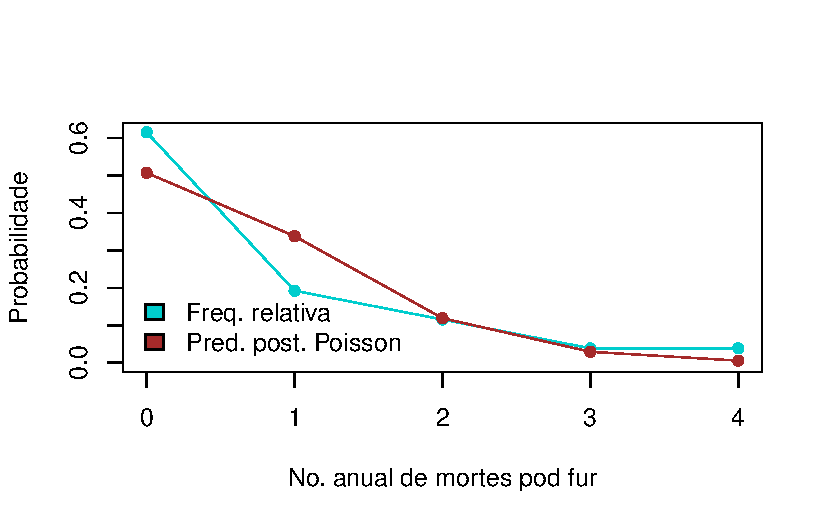
\includegraphics{misturas_files/figure-pdf/unnamed-chunk-2-1.pdf}

}

\end{figure}

\begin{Shaded}
\begin{Highlighting}[]
\CommentTok{\# hiperparâmetros para rho}
\NormalTok{a }\OtherTok{=}\NormalTok{ b }\OtherTok{=} \DecValTok{1}

\CommentTok{\# hiperparâmetros para theta}
\NormalTok{r}\OtherTok{=}\NormalTok{.}\DecValTok{1}
\NormalTok{s}\OtherTok{=}\NormalTok{.}\DecValTok{1}

\CommentTok{\# tamanho da amostra}
\NormalTok{n }\OtherTok{\textless{}{-}} \FunctionTok{length}\NormalTok{(fur) }

\CommentTok{\# valores iniciais da cadeia}
\NormalTok{theta }\OtherTok{\textless{}{-}} \FunctionTok{mean}\NormalTok{(fur)}
\NormalTok{rho }\OtherTok{\textless{}{-}} \FunctionTok{mean}\NormalTok{(fur }\SpecialCharTok{==} \DecValTok{0}\NormalTok{)}

\CommentTok{\# amostrador de Gibbs}
\NormalTok{B }\OtherTok{\textless{}{-}} \DecValTok{50000}
\ControlFlowTok{for}\NormalTok{(i }\ControlFlowTok{in} \DecValTok{1}\SpecialCharTok{:}\NormalTok{B)\{}
  \CommentTok{\# simulando z}
\NormalTok{  z }\OtherTok{\textless{}{-}} \ConstantTok{NULL}
\NormalTok{  prob }\OtherTok{\textless{}{-}}\NormalTok{ rho[i]}\SpecialCharTok{/}\NormalTok{ ( (}\DecValTok{1}\SpecialCharTok{{-}}\NormalTok{rho[i])}\SpecialCharTok{*}\FunctionTok{dpois}\NormalTok{(}\DecValTok{0}\NormalTok{,theta[i]) }\SpecialCharTok{+}\NormalTok{ rho[i])}
  \ControlFlowTok{for}\NormalTok{(j }\ControlFlowTok{in} \DecValTok{1}\SpecialCharTok{:}\NormalTok{n)\{}
    \ControlFlowTok{if}\NormalTok{(fur[j] }\SpecialCharTok{\textgreater{}}\DecValTok{0}\NormalTok{)\{ z[j] }\OtherTok{\textless{}{-}} \DecValTok{0}\NormalTok{\} }\ControlFlowTok{else}\NormalTok{\{}
\NormalTok{      z[j] }\OtherTok{\textless{}{-}} \FunctionTok{rbinom}\NormalTok{(}\DecValTok{1}\NormalTok{,}\DecValTok{1}\NormalTok{,prob)}
\NormalTok{    \}}
\NormalTok{  \}}

  \CommentTok{\# simulando rho}
\NormalTok{  rho[i}\SpecialCharTok{+}\DecValTok{1}\NormalTok{] }\OtherTok{\textless{}{-}} \FunctionTok{rbeta}\NormalTok{( }\DecValTok{1}\NormalTok{, a }\SpecialCharTok{+} \FunctionTok{sum}\NormalTok{( z }\SpecialCharTok{*}\NormalTok{ (fur }\SpecialCharTok{==} \DecValTok{0}\NormalTok{)) , n}\SpecialCharTok{{-}} \FunctionTok{sum}\NormalTok{(z)}\SpecialCharTok{+}\NormalTok{ b )}
  
  \CommentTok{\# simulando theta}
\NormalTok{  theta[i}\SpecialCharTok{+}\DecValTok{1}\NormalTok{] }\OtherTok{\textless{}{-}} \FunctionTok{rgamma}\NormalTok{(}\DecValTok{1}\NormalTok{, }\FunctionTok{sum}\NormalTok{( fur}\SpecialCharTok{*}\NormalTok{(}\DecValTok{1}\SpecialCharTok{{-}}\NormalTok{z) ) }\SpecialCharTok{+}\NormalTok{ r,  n }\SpecialCharTok{{-}} \FunctionTok{sum}\NormalTok{(z) }\SpecialCharTok{+}\NormalTok{ s)}
\NormalTok{\}}
\end{Highlighting}
\end{Shaded}

Vamos descartar a metade das simulações e usar um \textbf{thinning}
igual a 15:

\begin{Shaded}
\begin{Highlighting}[]
\NormalTok{theta\_sim }\OtherTok{\textless{}{-}}\NormalTok{ theta[}\FunctionTok{seq}\NormalTok{(B}\SpecialCharTok{/}\DecValTok{2}\NormalTok{,B,}\DecValTok{15}\NormalTok{)]}
\NormalTok{rho\_sim }\OtherTok{\textless{}{-}}\NormalTok{ rho[}\FunctionTok{seq}\NormalTok{(B}\SpecialCharTok{/}\DecValTok{2}\NormalTok{,B,}\DecValTok{15}\NormalTok{)]}

\NormalTok{oo }\OtherTok{\textless{}{-}} \FunctionTok{par}\NormalTok{(}\AttributeTok{mfrow=}\FunctionTok{c}\NormalTok{(}\DecValTok{2}\NormalTok{,}\DecValTok{2}\NormalTok{))}
\FunctionTok{ts.plot}\NormalTok{(theta\_sim, }\AttributeTok{lwd =} \DecValTok{2}\NormalTok{)}
\FunctionTok{ts.plot}\NormalTok{(rho\_sim, }\AttributeTok{lwd =} \DecValTok{2}\NormalTok{)}
\FunctionTok{acf}\NormalTok{(theta\_sim)}
\FunctionTok{acf}\NormalTok{(rho\_sim)}
\end{Highlighting}
\end{Shaded}

\begin{figure}[H]

{\centering 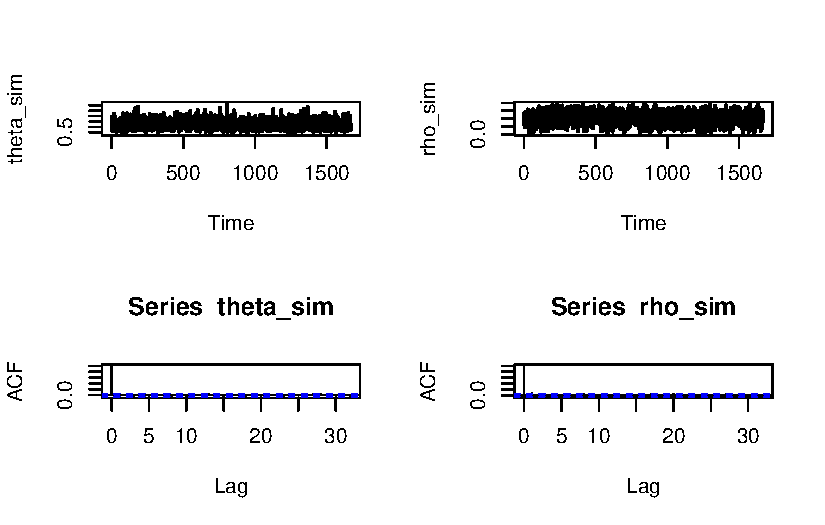
\includegraphics{misturas_files/figure-pdf/unnamed-chunk-4-1.pdf}

}

\end{figure}

Vamos estimar as probabilidade de ocorrerem \(k\) mortes via preditiva
posteriori:

\begin{Shaded}
\begin{Highlighting}[]
\CommentTok{\# tamanho do vetor simulado}
\NormalTok{Bs }\OtherTok{\textless{}{-}} \FunctionTok{length}\NormalTok{(theta\_sim)}

\NormalTok{x\_til }\OtherTok{\textless{}{-}} \FunctionTok{array}\NormalTok{( }\ConstantTok{NA\_real\_}\NormalTok{, }\FunctionTok{c}\NormalTok{(Bs,n))}
\ControlFlowTok{for}\NormalTok{(j }\ControlFlowTok{in} \DecValTok{1}\SpecialCharTok{:}\NormalTok{Bs)\{}
\NormalTok{  z }\OtherTok{\textless{}{-}} \FunctionTok{rbinom}\NormalTok{( n, }\DecValTok{1}\NormalTok{, rho\_sim[j])}
\NormalTok{  x\_til[j,] }\OtherTok{\textless{}{-}}\NormalTok{ (}\DecValTok{1}\SpecialCharTok{{-}}\NormalTok{z)}\SpecialCharTok{*}\FunctionTok{rpois}\NormalTok{(n, theta\_sim[j])}
\NormalTok{\}}

\CommentTok{\# probabilidades estimadas via ZIP}
\NormalTok{p\_zip }\OtherTok{\textless{}{-}} \FunctionTok{prop.table}\NormalTok{(}\FunctionTok{table}\NormalTok{(x\_til))}

\NormalTok{p\_zip}
\end{Highlighting}
\end{Shaded}

\begin{verbatim}
x_til
           0            1            2            3            4            5 
6.112085e-01 1.979373e-01 1.149232e-01 5.050528e-02 1.771953e-02 5.583499e-03 
           6            7            8            9 
1.707351e-03 3.460846e-04 2.307231e-05 4.614462e-05 
\end{verbatim}

Abaixo mostramos as probabilidades preditas do modelo ZIP, do modelo
Poisson a e frequência relativa.

\begin{Shaded}
\begin{Highlighting}[]
\NormalTok{r1 }\OtherTok{\textless{}{-}} \FunctionTok{sum}\NormalTok{(fur)}
\NormalTok{s1 }\OtherTok{\textless{}{-}} \FunctionTok{length}\NormalTok{(fur)}
\FunctionTok{plot}\NormalTok{(}\FunctionTok{table}\NormalTok{(fur)}\SpecialCharTok{/}\NormalTok{s1, }\AttributeTok{type=} \StringTok{\textquotesingle{}p\textquotesingle{}}\NormalTok{, }\AttributeTok{xlab=}\StringTok{\textquotesingle{}No. anual de mortes pod fur\textquotesingle{}}\NormalTok{, }\AttributeTok{ylab =} \StringTok{\textquotesingle{}Probabilidade\textquotesingle{}}\NormalTok{, }\AttributeTok{col =} \StringTok{\textquotesingle{}cyan3\textquotesingle{}}\NormalTok{, }\AttributeTok{pch=}\DecValTok{16}\NormalTok{)}
\FunctionTok{lines}\NormalTok{(}\DecValTok{0}\SpecialCharTok{:}\DecValTok{4}\NormalTok{,}\FunctionTok{table}\NormalTok{(fur)}\SpecialCharTok{/}\NormalTok{s1, }\AttributeTok{col =} \StringTok{\textquotesingle{}cyan3\textquotesingle{}}\NormalTok{)}
\FunctionTok{points}\NormalTok{(}\DecValTok{0}\SpecialCharTok{:}\DecValTok{4}\NormalTok{, }\FunctionTok{dnbinom}\NormalTok{(}\DecValTok{0}\SpecialCharTok{:}\DecValTok{4}\NormalTok{, }\AttributeTok{size =}\NormalTok{ r1, }\AttributeTok{prob =}\NormalTok{ s1}\SpecialCharTok{/}\NormalTok{(}\DecValTok{1}\SpecialCharTok{+}\NormalTok{s1)), }\AttributeTok{pch=}\DecValTok{16}\NormalTok{, }\AttributeTok{col =} \StringTok{\textquotesingle{}brown\textquotesingle{}}\NormalTok{)}
\FunctionTok{lines}\NormalTok{(}\DecValTok{0}\SpecialCharTok{:}\DecValTok{4}\NormalTok{, }\FunctionTok{dnbinom}\NormalTok{(}\DecValTok{0}\SpecialCharTok{:}\DecValTok{4}\NormalTok{, }\AttributeTok{size =}\NormalTok{ r1, }\AttributeTok{prob =}\NormalTok{ s1}\SpecialCharTok{/}\NormalTok{(}\DecValTok{1}\SpecialCharTok{+}\NormalTok{s1)), }\AttributeTok{col =} \StringTok{\textquotesingle{}brown\textquotesingle{}}\NormalTok{)}
\FunctionTok{points}\NormalTok{(}\FunctionTok{names}\NormalTok{(p\_zip),p\_zip, }\AttributeTok{pch=}\DecValTok{16}\NormalTok{,}\AttributeTok{col =} \StringTok{\textquotesingle{}magenta\textquotesingle{}}\NormalTok{)}
\FunctionTok{lines}\NormalTok{(}\FunctionTok{names}\NormalTok{(p\_zip),p\_zip,}\AttributeTok{col =} \StringTok{\textquotesingle{}magenta\textquotesingle{}}\NormalTok{)}

\FunctionTok{legend}\NormalTok{(}\StringTok{\textquotesingle{}bottomleft\textquotesingle{}}\NormalTok{,}\FunctionTok{c}\NormalTok{(}\StringTok{\textquotesingle{}Freq. relativa\textquotesingle{}}\NormalTok{,}\StringTok{\textquotesingle{}Pred. post. Poisson\textquotesingle{}}\NormalTok{, }\StringTok{\textquotesingle{}Pred. post. ZIP\textquotesingle{}}\NormalTok{), }\AttributeTok{fill=}\FunctionTok{c}\NormalTok{(}\StringTok{\textquotesingle{}cyan3\textquotesingle{}}\NormalTok{,}\StringTok{\textquotesingle{}brown\textquotesingle{}}\NormalTok{, }\StringTok{\textquotesingle{}magenta\textquotesingle{}}\NormalTok{), }\AttributeTok{bty=}\StringTok{\textquotesingle{}n\textquotesingle{}}\NormalTok{)}
\end{Highlighting}
\end{Shaded}

\begin{figure}[H]

{\centering 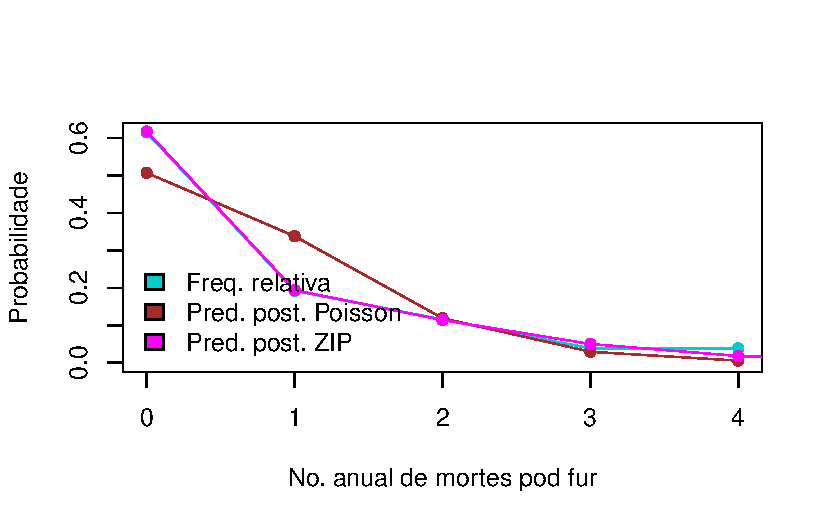
\includegraphics{misturas_files/figure-pdf/unnamed-chunk-6-1.pdf}

}

\end{figure}

\hypertarget{exercuxedcio}{%
\section{Exercício}\label{exercuxedcio}}

Abaixo, segue o número anual de tornados em Lafayette Parish, Louisiana,
entre 1950 e 2012.

\begin{Shaded}
\begin{Highlighting}[]
\NormalTok{tor }\OtherTok{\textless{}{-}} \FunctionTok{c}\NormalTok{(}\DecValTok{0}\NormalTok{, }\DecValTok{0}\NormalTok{,}\DecValTok{0}\NormalTok{, }\DecValTok{1}\NormalTok{, }\DecValTok{0}\NormalTok{, }\DecValTok{0}\NormalTok{, }\DecValTok{0}\NormalTok{, }\DecValTok{1}\NormalTok{, }\DecValTok{0}\NormalTok{, }\DecValTok{0}\NormalTok{,}
\DecValTok{1}\NormalTok{, }\DecValTok{0}\NormalTok{, }\DecValTok{0}\NormalTok{, }\DecValTok{0}\NormalTok{, }\DecValTok{1}\NormalTok{, }\DecValTok{1}\NormalTok{, }\DecValTok{0}\NormalTok{, }\DecValTok{0}\NormalTok{, }\DecValTok{0}\NormalTok{, }\DecValTok{2}\NormalTok{,}
\DecValTok{0}\NormalTok{, }\DecValTok{0}\NormalTok{, }\DecValTok{0}\NormalTok{, }\DecValTok{0}\NormalTok{, }\DecValTok{1}\NormalTok{, }\DecValTok{3}\NormalTok{, }\DecValTok{0}\NormalTok{, }\DecValTok{2}\NormalTok{, }\DecValTok{1}\NormalTok{, }\DecValTok{0}\NormalTok{,}
\DecValTok{1}\NormalTok{, }\DecValTok{0}\NormalTok{, }\DecValTok{0}\NormalTok{, }\DecValTok{1}\NormalTok{, }\DecValTok{0}\NormalTok{, }\DecValTok{1}\NormalTok{, }\DecValTok{0}\NormalTok{, }\DecValTok{0}\NormalTok{, }\DecValTok{2}\NormalTok{, }\DecValTok{1}\NormalTok{,}
\DecValTok{0}\NormalTok{, }\DecValTok{1}\NormalTok{, }\DecValTok{2}\NormalTok{, }\DecValTok{0}\NormalTok{, }\DecValTok{0}\NormalTok{, }\DecValTok{1}\NormalTok{, }\DecValTok{0}\NormalTok{, }\DecValTok{1}\NormalTok{, }\DecValTok{2}\NormalTok{, }\DecValTok{0}\NormalTok{,}
\DecValTok{0}\NormalTok{, }\DecValTok{0}\NormalTok{, }\DecValTok{3}\NormalTok{, }\DecValTok{0}\NormalTok{, }\DecValTok{2}\NormalTok{, }\DecValTok{0}\NormalTok{, }\DecValTok{1}\NormalTok{, }\DecValTok{1}\NormalTok{, }\DecValTok{3}\NormalTok{, }\DecValTok{0}\NormalTok{,}
\DecValTok{1}\NormalTok{, }\DecValTok{1}\NormalTok{, }\DecValTok{1}\NormalTok{)}
\end{Highlighting}
\end{Shaded}

\begin{itemize}
\item
  Ajuste o modelo Poisson.
\item
  Ajuste o modelo Poisson inflado de zeros.
\end{itemize}

\bookmarksetup{startatroot}

\hypertarget{o-modelo-poisson-revisitado}{%
\chapter{O modelo Poisson
revisitado}\label{o-modelo-poisson-revisitado}}

\hypertarget{verossimilhanuxe7a-prioris-e-posterioris}{%
\section{Verossimilhança, prioris e
posterioris}\label{verossimilhanuxe7a-prioris-e-posterioris}}

Dizemos que \(X|\theta\) tem distribuição Poisson se sua função de
probabilidade é dada por \[f(x|\theta)=\frac{e^{-\theta}\theta^x}{x!},\]
onde \(x=0,1,\ldots\) e \(\theta>0\). O parâmetro \(\theta\) é
denominado taxa. Para este modelo \[E(X|\theta)=Var(X|\theta)=\theta.\]

Esta é uma das distribuições para contagens mais importantes. A
verossimilhança deste modelo, para uma amostra de vaiid, é dada por
\[L(\theta)=\frac{e^{-n\theta}\theta^{\sum_{i=1}^{n}x_i}}{\prod_{i=1}^{n}x_i!}.\]
O modelo Poisson pertence à família exponencial e sua \textit{priori}
conjugada é \(\theta\sim\hbox{Gama}(r,s)\), onde \(r\) e \(s\) podem ser
interpretados como o total da contagem e o tamanho da amostra
\textit{a priori}.

Neste caso, a \textit{posteriori} é
\(\hbox{Gama}(r+\sum_{i=1}^n x_i+r, s+n)\).

A média da \textit{posteriori} é
\[E(\theta|\mathbf{x})=\frac{\sum_{i=1}^{n}x_i+r}{n+s}=\frac{n}{n+s}\bar{x}+\frac{s}{n+s}E(\theta),\]
onde fica claro que este estimador é uma média ponderada das informações
provenientes das duas fontes de informação (sendo \(\bar{x}\) a
estimativa de máxima verossimilhança e \(E(\theta)\) a média
\textit{a priori}).

Se \(n\gg s\), então a média a posteriori dará maior peso para a
informação dos dados.

A informação de Fisher é \[\mathcal{I}(\theta)=\frac{1}{\theta}\]

Assim, a priori de Jeffreys é dada por
\[f(\theta)\propto \theta^{-\frac{1}{2}},\] sendo, portanto, uma priori
imprópria. Contudo,
\[f(\theta|\mathbf{x})\propto e^{-n\theta}\theta^{\sum_{i=1}^{n}x_i} \theta^{-\frac{1}{2}},\]
logo, a posteriori é própria, tendo distribuição
\(Gama(\sum_{i=1}^{n}x_i+1/2,n)\).

Considere a posteriori \(\theta|\mathbf{x}\sim\hbox{Gama}(r_1,s_1)\).
Podemos retirar uma amostra da preditiva \textit{a posteriori} do
seguinte modo:

\begin{enumerate}
\def\labelenumi{\arabic{enumi}.}
\tightlist
\item
  Gere \(\theta_j\sim\hbox{Gama}(r_1,s_1)\)
\end{enumerate}

2.Gere \(\tilde{\mathbf{x}}\sim\hbox{Poisson}(\theta_j)\).

\hypertarget{o-modelo-poisson-para-taxas}{%
\section{O modelo Poisson para
taxas}\label{o-modelo-poisson-para-taxas}}

A taxa é o cociente entre o número de casos de um evento em determinado
intervalo de tempo e a população em risco, definida em um espaço e no
mesmo intervalo de tempo (``pessoas-tempo'\,'). Note que, pela
definição, a taxa é uma estatística.

Seja \(n\) o tamanho da população no espaço/tempo e seja \(y\) o número
de casos do evento de interesse. Então,

\[\hbox{taxa} = \frac{y}{n}\]

Contudo, como \(n\) tende a ser muito maior que \(y\), é comum reportar
a taxa vezes \(10^k\), para algum \(k>0\).

Exemplo: Segundo o Anuário de Segurança Pública 2022, em 2021 houveram
68.885 casos de estupro. Considerando uma população de 212,7 milhões de
habitantes, a taxa de estupro para aquele ano foi de
\[\frac{68.885}{212.700.000}=3,23\times 10^{-4}\] casos por pessoa-ano.
Como \(n\) tende a ser maior que \(y\), é comum considerar.

Multiplicando a taxa por \(10^5\), temos uma taxa de 32,3 casos para
cada 100.000 habitantes.

Agora,considere que \(\theta\) é o parâmetro taxa. Então,

\[\hat{\theta}=\frac{y}{n}\] é a estimativa para \(\theta\). Como \(y\)
é uma contagem, é razoável supor que \[\theta =\frac{1}{n}E(Y|\theta).\]
e um modelo possível seria \(y|\theta\sim\hbox{Poisson}(\theta n)\).

Agora, considere que uma população está particionada em \(m\)
localidades. Para um dado intervalo de tempo, sejam \(n_i\) e \(y_i\) a
população da localidade \(i\) e seu respectivo número de casos
observados. Suponha ainda que a taxa \(\theta\) é comum para a pooulação
e que \(y_i\) é condicionalmente independente de \(y_j\) dado
\(\theta\). Assumindo a distribuição Poisson, teremos

\[L(\theta)=\prod_{i=1}^m\frac{e^{-\theta n_i}(\theta n_i)^{y_i}}{y_i!}\varpropto \theta^{\sum_{i=1}^m y_i}e^{-\theta \sum_{i=1}^m n_i}=\theta^{\sum_{i=1}^n y_i}e^{-\theta N},\]
onde \(N=\sum_{i=1}^m n_i\) é o tamanho da população. Como a
verossimilhança pertence à família exponencial, temos que o modelo
Gama\((a,b)\) é conjugado gerando a posteriori

\[\theta|\mathbf{y}\sim\hbox{Gama}\left(\sum_{i=1}^{m}y_i+a,N+b\right).\]

A prioris impróprias \(\pi(\theta)\varpropto \theta^{-1}\) e
\(\pi(\theta)\varpropto \theta^{-1/2}\) geram, respectivamente, as
posterioris \(\hbox{Gama}(\sum_{i=1}^m y_i,N)\) e
\(\hbox{Gama}(\sum_{i=1}^m y_i+1/2,N)\).

\hypertarget{exemplo-1-crime-de-estupro-de-vulneruxe1vel-no-interior-do-amazonas}{%
\section{Exemplo 1: crime de estupro de vulnerável no interior do
Amazonas}\label{exemplo-1-crime-de-estupro-de-vulneruxe1vel-no-interior-do-amazonas}}

Os dados a seguir foram cedidos pelo Observatório de Violência de Gênero
no Amazonas e compreendem os anos entre 2010 e 2012.

\begin{longtable}[]{@{}lll@{}}
\toprule\noalign{}
Cidade & vitimas & Populacao feminina \\
\midrule\noalign{}
\endhead
\bottomrule\noalign{}
\endlastfoot
Amatura & 3 & 639 \\
Atalaia do Norte & 6 & 905 \\
Barreirinha & 12 & 1899 \\
Benjamin Constant & 2 & 2036 \\
Boa Vista do Ramos & 6 & 1060 \\
Fonte Boa & 0 & 1438 \\
Jutai & 1 & 1143 \\
Maues & 13 & 3421 \\
Nhamunda & 9 & 1168 \\
Parintins & 20 & 6700 \\
Santo Antonio do Ica & 7 & 1608 \\
Sao Paulo de Olivenca & 5 & 2033 \\
Tabatinga & 8 & 3095 \\
Tonantins & 1 & 1186 \\
\end{longtable}

Considerando a priori \(\pi(\theta)\varpropto \theta^{-1/2}\) teremos:

\begin{Shaded}
\begin{Highlighting}[]
\CommentTok{\# banco de dados}
\NormalTok{casos }\OtherTok{\textless{}{-}} \FunctionTok{c}\NormalTok{( }\DecValTok{3}\NormalTok{, }\DecValTok{6}\NormalTok{, }\DecValTok{12}\NormalTok{, }\DecValTok{2}\NormalTok{, }\DecValTok{6}\NormalTok{, }\DecValTok{0}\NormalTok{, }\DecValTok{1}\NormalTok{, }\DecValTok{13}\NormalTok{, }\DecValTok{9}\NormalTok{, }\DecValTok{20}\NormalTok{, }\DecValTok{7}\NormalTok{, }\DecValTok{5}\NormalTok{, }\DecValTok{8}\NormalTok{, }\DecValTok{1}\NormalTok{ )   }

\NormalTok{pop }\OtherTok{\textless{}{-}} \FunctionTok{c}\NormalTok{(}\DecValTok{639}\NormalTok{, }\DecValTok{905}\NormalTok{, }\DecValTok{1899}\NormalTok{, }\DecValTok{2036}\NormalTok{, }\DecValTok{1060}\NormalTok{, }\DecValTok{1438}\NormalTok{, }\DecValTok{1143}\NormalTok{, }\DecValTok{3421}\NormalTok{, }\DecValTok{1168}\NormalTok{, }\DecValTok{6700}\NormalTok{, }\DecValTok{1608}\NormalTok{, }\DecValTok{2033}\NormalTok{, }\DecValTok{3095}\NormalTok{, }\DecValTok{1186}\NormalTok{)}
\NormalTok{pop }\OtherTok{\textless{}{-}}\NormalTok{ pop}\SpecialCharTok{/}\DecValTok{10}\SpecialCharTok{\^{}}\DecValTok{5}

\NormalTok{municipios }\OtherTok{\textless{}{-}} \FunctionTok{c}\NormalTok{( }\StringTok{\textquotesingle{}Amatura\textquotesingle{}}\NormalTok{, }\StringTok{\textquotesingle{}Atl.Norte\textquotesingle{}}\NormalTok{, }\StringTok{\textquotesingle{}Barr\textquotesingle{}}\NormalTok{, }\StringTok{\textquotesingle{}BC\textquotesingle{}}\NormalTok{,}\StringTok{\textquotesingle{}BV Ramos\textquotesingle{}}\NormalTok{, }\StringTok{\textquotesingle{}Fonte B\textquotesingle{}}\NormalTok{, }\StringTok{\textquotesingle{}Jutai\textquotesingle{}}\NormalTok{, }\StringTok{\textquotesingle{}Maues\textquotesingle{}}\NormalTok{, }\StringTok{\textquotesingle{}Nhamunda\textquotesingle{}}\NormalTok{, }\StringTok{\textquotesingle{}Parintins\textquotesingle{}}\NormalTok{, }\StringTok{\textquotesingle{}StoIca\textquotesingle{}}\NormalTok{, }\StringTok{\textquotesingle{}SP Olivenca\textquotesingle{}}\NormalTok{, }\StringTok{\textquotesingle{}Tbt\textquotesingle{}}\NormalTok{,}\StringTok{\textquotesingle{}Tonantins\textquotesingle{}}\NormalTok{)}
\end{Highlighting}
\end{Shaded}

\begin{Shaded}
\begin{Highlighting}[]
\CommentTok{\# posteriori}
\NormalTok{a\_post }\OtherTok{\textless{}{-}} \FunctionTok{sum}\NormalTok{(casos) }\SpecialCharTok{+}\NormalTok{ .}\DecValTok{5}
\NormalTok{b\_post }\OtherTok{\textless{}{-}} \FunctionTok{sum}\NormalTok{(pop)}

\FunctionTok{curve}\NormalTok{(}\FunctionTok{dgamma}\NormalTok{(x,a\_post,b\_post),}\DecValTok{230}\NormalTok{,}\DecValTok{450}\NormalTok{ ,}\AttributeTok{lwd =} \DecValTok{2}\NormalTok{, }\AttributeTok{xlab =} \FunctionTok{expression}\NormalTok{(theta), }\AttributeTok{ylab =} \StringTok{\textquotesingle{}densidade a posteriori\textquotesingle{}}\NormalTok{ )}
\end{Highlighting}
\end{Shaded}

\begin{figure}[H]

{\centering 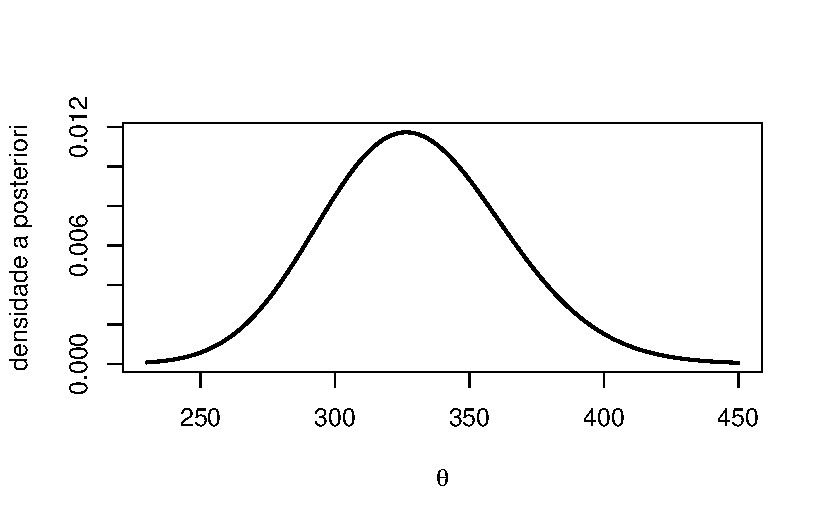
\includegraphics{poisson_files/figure-pdf/unnamed-chunk-2-1.pdf}

}

\end{figure}

Abaixo, simulamos 50.000 amostras da preditiva a posteriori

\begin{Shaded}
\begin{Highlighting}[]
\NormalTok{B }\OtherTok{\textless{}{-}} \DecValTok{50000} \CommentTok{\# número de simulações da preditiva a posteriori}
\NormalTok{m }\OtherTok{\textless{}{-}} \FunctionTok{length}\NormalTok{(casos)}

\NormalTok{pred\_mun }\OtherTok{\textless{}{-}} \ConstantTok{NULL}
\ControlFlowTok{for}\NormalTok{(i }\ControlFlowTok{in} \DecValTok{1}\SpecialCharTok{:}\DecValTok{5000}\NormalTok{)\{}
\NormalTok{  theta }\OtherTok{\textless{}{-}} \FunctionTok{rgamma}\NormalTok{(}\DecValTok{1}\NormalTok{, }\FunctionTok{sum}\NormalTok{(casos) }\SpecialCharTok{+}\NormalTok{ .}\DecValTok{5}\NormalTok{, }\FunctionTok{sum}\NormalTok{(pop))}
\NormalTok{  pred\_mun }\OtherTok{\textless{}{-}} \FunctionTok{rbind}\NormalTok{(pred\_mun, }\FunctionTok{rpois}\NormalTok{(m , theta }\SpecialCharTok{*}\NormalTok{ pop))}
\NormalTok{\}}

\NormalTok{pred\_mun }\OtherTok{\textless{}{-}} \FunctionTok{data.frame}\NormalTok{(pred\_mun)}
\FunctionTok{names}\NormalTok{(pred\_mun) }\OtherTok{\textless{}{-}}\NormalTok{ municipios}
\FunctionTok{boxplot}\NormalTok{(pred\_mun)}
\FunctionTok{points}\NormalTok{(}\DecValTok{1}\SpecialCharTok{:}\DecValTok{14}\NormalTok{,casos, }\AttributeTok{pch=}\DecValTok{16}\NormalTok{,}\AttributeTok{cex =} \FloatTok{1.2}\NormalTok{, }\AttributeTok{col =}\StringTok{\textquotesingle{}tomato\textquotesingle{}}\NormalTok{)}
\end{Highlighting}
\end{Shaded}

\begin{figure}[H]

{\centering 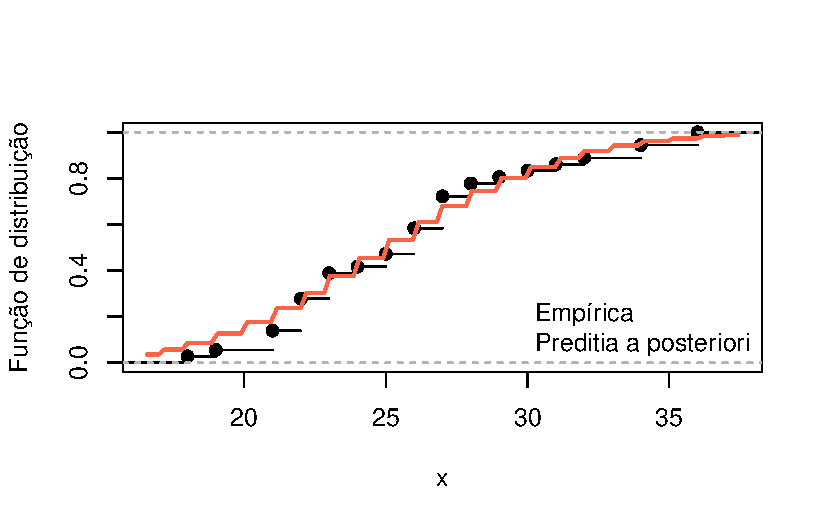
\includegraphics{poisson_files/figure-pdf/unnamed-chunk-3-1.pdf}

}

\end{figure}

\begin{Shaded}
\begin{Highlighting}[]
\NormalTok{oo }\OtherTok{\textless{}{-}} \FunctionTok{par}\NormalTok{()}
\NormalTok{mat }\OtherTok{\textless{}{-}} \FunctionTok{matrix}\NormalTok{(}\DecValTok{1}\SpecialCharTok{:}\NormalTok{m,}\AttributeTok{ncol=}\DecValTok{2}\NormalTok{)}
\NormalTok{mat }\OtherTok{\textless{}{-}} \FunctionTok{rbind}\NormalTok{(mat, }\FunctionTok{c}\NormalTok{(}\DecValTok{15}\NormalTok{,}\DecValTok{16}\NormalTok{))}
\FunctionTok{layout}\NormalTok{(mat, }\AttributeTok{heights =} \FunctionTok{rep}\NormalTok{(}\DecValTok{1}\NormalTok{,}\DecValTok{14}\NormalTok{,.}\DecValTok{5}\NormalTok{,.}\DecValTok{5}\NormalTok{))}

\ControlFlowTok{for}\NormalTok{(i }\ControlFlowTok{in} \DecValTok{1}\SpecialCharTok{:}\NormalTok{m)\{}
\NormalTok{  freq }\OtherTok{\textless{}{-}} \FunctionTok{prop.table}\NormalTok{( }\FunctionTok{table}\NormalTok{(pred\_mun[,i]) )}
  \FunctionTok{par}\NormalTok{(}\AttributeTok{mar =} \FunctionTok{c}\NormalTok{(}\DecValTok{1}\NormalTok{,}\DecValTok{5}\NormalTok{,}\DecValTok{1}\NormalTok{,}\DecValTok{1}\NormalTok{), }\AttributeTok{cex =}\NormalTok{ .}\DecValTok{8}\NormalTok{)}
  \FunctionTok{plot.new}\NormalTok{()}
  \FunctionTok{plot.window}\NormalTok{(}\AttributeTok{xlim=}\FunctionTok{c}\NormalTok{(}\DecValTok{0}\NormalTok{,}\DecValTok{46}\NormalTok{), }\AttributeTok{ylim =} \FunctionTok{c}\NormalTok{(}\DecValTok{0}\NormalTok{,.}\DecValTok{3}\NormalTok{))}
  \FunctionTok{points}\NormalTok{(}\FunctionTok{as.numeric}\NormalTok{(}\FunctionTok{names}\NormalTok{(freq)), freq, }\AttributeTok{type=}\StringTok{\textquotesingle{}h\textquotesingle{}}\NormalTok{, }\AttributeTok{lwd =} \DecValTok{2}\NormalTok{)}
  \FunctionTok{title}\NormalTok{(}\AttributeTok{ylab=}\NormalTok{municipios[i])}
  \FunctionTok{points}\NormalTok{(casos[i],}\DecValTok{0}\NormalTok{,}\AttributeTok{pch=}\DecValTok{16}\NormalTok{,}\AttributeTok{col=}\StringTok{\textquotesingle{}tomato\textquotesingle{}}\NormalTok{,}\AttributeTok{cex=} \FloatTok{1.2}\NormalTok{)}
  
\NormalTok{\}}
  \FunctionTok{par}\NormalTok{(}\AttributeTok{mar =} \FunctionTok{c}\NormalTok{(}\DecValTok{2}\NormalTok{,}\DecValTok{5}\NormalTok{,}\DecValTok{0}\NormalTok{,}\DecValTok{1}\NormalTok{))}
  \FunctionTok{plot.new}\NormalTok{()}
  \FunctionTok{plot.window}\NormalTok{(}\AttributeTok{xlim=}\FunctionTok{c}\NormalTok{(}\DecValTok{0}\NormalTok{,}\DecValTok{46}\NormalTok{), }\AttributeTok{ylim =} \FunctionTok{c}\NormalTok{(}\DecValTok{0}\NormalTok{,.}\DecValTok{1}\NormalTok{))}
  \FunctionTok{segments}\NormalTok{(}\DecValTok{0}\NormalTok{,.}\DecValTok{05}\NormalTok{,}\DecValTok{46}\NormalTok{,.}\DecValTok{05}\NormalTok{,}\AttributeTok{lwd=}\DecValTok{2}\NormalTok{)}
 \ControlFlowTok{for}\NormalTok{(j }\ControlFlowTok{in} \FunctionTok{seq}\NormalTok{(}\DecValTok{0}\NormalTok{,}\DecValTok{45}\NormalTok{,}\DecValTok{5}\NormalTok{))\{}
    \FunctionTok{segments}\NormalTok{(j,.}\DecValTok{05}\NormalTok{,j,.}\DecValTok{03}\NormalTok{)}
    \FunctionTok{text}\NormalTok{(j,.}\DecValTok{01}\NormalTok{,j)}
\NormalTok{  \}}
    \FunctionTok{par}\NormalTok{(}\AttributeTok{mar =} \FunctionTok{c}\NormalTok{(}\DecValTok{2}\NormalTok{,}\DecValTok{5}\NormalTok{,}\DecValTok{0}\NormalTok{,}\DecValTok{1}\NormalTok{))}
  \FunctionTok{plot.new}\NormalTok{()}
  \FunctionTok{plot.window}\NormalTok{(}\AttributeTok{xlim=}\FunctionTok{c}\NormalTok{(}\DecValTok{0}\NormalTok{,}\DecValTok{46}\NormalTok{), }\AttributeTok{ylim =} \FunctionTok{c}\NormalTok{(}\DecValTok{0}\NormalTok{,.}\DecValTok{1}\NormalTok{))}
  \FunctionTok{segments}\NormalTok{(}\DecValTok{0}\NormalTok{,.}\DecValTok{05}\NormalTok{,}\DecValTok{46}\NormalTok{,.}\DecValTok{05}\NormalTok{,}\AttributeTok{lwd=}\DecValTok{2}\NormalTok{)}
  \ControlFlowTok{for}\NormalTok{(j }\ControlFlowTok{in} \FunctionTok{seq}\NormalTok{(}\DecValTok{0}\NormalTok{,}\DecValTok{45}\NormalTok{,}\DecValTok{5}\NormalTok{))\{}
    \FunctionTok{segments}\NormalTok{(j,.}\DecValTok{05}\NormalTok{,j,.}\DecValTok{03}\NormalTok{)}
    \FunctionTok{text}\NormalTok{(j,.}\DecValTok{01}\NormalTok{,j)}
\NormalTok{  \}}
\end{Highlighting}
\end{Shaded}

\begin{figure}[H]

{\centering 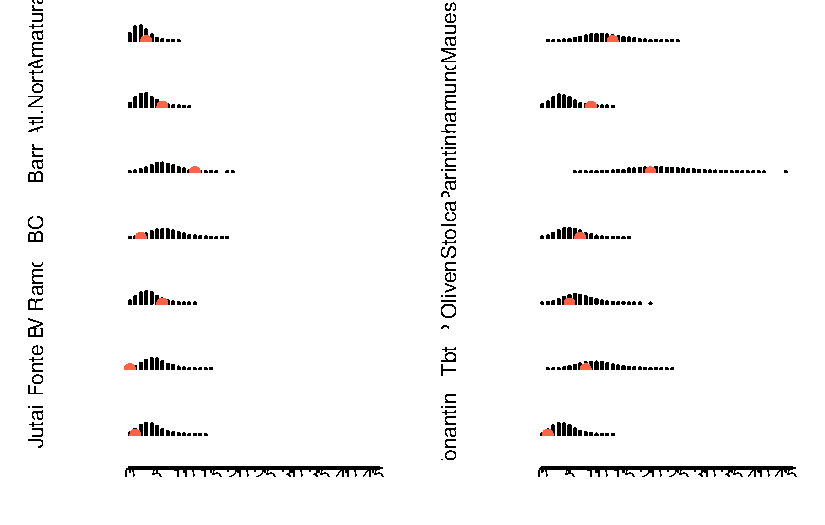
\includegraphics{poisson_files/figure-pdf/unnamed-chunk-4-1.pdf}

}

\end{figure}

\begin{Shaded}
\begin{Highlighting}[]
\FunctionTok{par}\NormalTok{(oo)}
\end{Highlighting}
\end{Shaded}

\begin{verbatim}
Warning in par(oo): parâmetro gráfico "cin" não pode ser especificado
\end{verbatim}

\begin{verbatim}
Warning in par(oo): parâmetro gráfico "cra" não pode ser especificado
\end{verbatim}

\begin{verbatim}
Warning in par(oo): parâmetro gráfico "csi" não pode ser especificado
\end{verbatim}

\begin{verbatim}
Warning in par(oo): parâmetro gráfico "cxy" não pode ser especificado
\end{verbatim}

\begin{verbatim}
Warning in par(oo): parâmetro gráfico "din" não pode ser especificado
\end{verbatim}

\begin{verbatim}
Warning in par(oo): parâmetro gráfico "page" não pode ser especificado
\end{verbatim}

\begin{Shaded}
\begin{Highlighting}[]
\NormalTok{p }\OtherTok{\textless{}{-}} \ConstantTok{NULL}
\ControlFlowTok{for}\NormalTok{(i }\ControlFlowTok{in} \DecValTok{1}\SpecialCharTok{:}\NormalTok{m)\{}
\NormalTok{p[i] }\OtherTok{\textless{}{-}} \DecValTok{2}\SpecialCharTok{*}\FunctionTok{min}\NormalTok{(}\FunctionTok{mean}\NormalTok{(pred\_mun[,i] }\SpecialCharTok{\textgreater{}}\NormalTok{ casos[i]),}
\FunctionTok{mean}\NormalTok{(pred\_mun[,i] }\SpecialCharTok{\textless{}}\NormalTok{ casos[i]))}
\NormalTok{\}}

\FunctionTok{data.frame}\NormalTok{(municipios,p)}
\end{Highlighting}
\end{Shaded}

\begin{verbatim}
    municipios      p
1      Amatura 0.3308
2    Atl.Norte 0.0836
3         Barr 0.0368
4           BC 0.0192
5     BV Ramos 0.1292
6      Fonte B 0.0000
7        Jutai 0.0476
8        Maues 0.4980
9     Nhamunda 0.0196
10   Parintins 0.6472
11      StoIca 0.3600
12 SP Olivenca 0.4388
13         Tbt 0.4156
14   Tonantins 0.0524
\end{verbatim}

\bookmarksetup{startatroot}

\hypertarget{references}{%
\chapter*{References}\label{references}}
\addcontentsline{toc}{chapter}{References}

\markboth{References}{References}

\hypertarget{refs}{}
\begin{CSLReferences}{0}{0}
\end{CSLReferences}



\end{document}
